% Options for packages loaded elsewhere
\PassOptionsToPackage{unicode}{hyperref}
\PassOptionsToPackage{hyphens}{url}
%
\documentclass[
  12pt,
  oneside]{book}
\usepackage{amsmath,amssymb}
\usepackage{lmodern}
\usepackage{ifxetex,ifluatex}
\ifnum 0\ifxetex 1\fi\ifluatex 1\fi=0 % if pdftex
  \usepackage[T1]{fontenc}
  \usepackage[utf8]{inputenc}
  \usepackage{textcomp} % provide euro and other symbols
\else % if luatex or xetex
  \usepackage{unicode-math}
  \defaultfontfeatures{Scale=MatchLowercase}
  \defaultfontfeatures[\rmfamily]{Ligatures=TeX,Scale=1}
\fi
% Use upquote if available, for straight quotes in verbatim environments
\IfFileExists{upquote.sty}{\usepackage{upquote}}{}
\IfFileExists{microtype.sty}{% use microtype if available
  \usepackage[]{microtype}
  \UseMicrotypeSet[protrusion]{basicmath} % disable protrusion for tt fonts
}{}
\makeatletter
\@ifundefined{KOMAClassName}{% if non-KOMA class
  \IfFileExists{parskip.sty}{%
    \usepackage{parskip}
  }{% else
    \setlength{\parindent}{0pt}
    \setlength{\parskip}{6pt plus 2pt minus 1pt}}
}{% if KOMA class
  \KOMAoptions{parskip=half}}
\makeatother
\usepackage{xcolor}
\IfFileExists{xurl.sty}{\usepackage{xurl}}{} % add URL line breaks if available
\IfFileExists{bookmark.sty}{\usepackage{bookmark}}{\usepackage{hyperref}}
\hypersetup{
  pdftitle={Tu Là Chuyển Nghiệp},
  pdfauthor={HT. Thích Thanh Từ},
  hidelinks,
  pdfcreator={LaTeX via pandoc}}
\urlstyle{same} % disable monospaced font for URLs
\usepackage{longtable,booktabs,array}
\usepackage{calc} % for calculating minipage widths
% Correct order of tables after \paragraph or \subparagraph
\usepackage{etoolbox}
\makeatletter
\patchcmd\longtable{\par}{\if@noskipsec\mbox{}\fi\par}{}{}
\makeatother
% Allow footnotes in longtable head/foot
\IfFileExists{footnotehyper.sty}{\usepackage{footnotehyper}}{\usepackage{footnote}}
\makesavenoteenv{longtable}
\usepackage{graphicx}
\makeatletter
\def\maxwidth{\ifdim\Gin@nat@width>\linewidth\linewidth\else\Gin@nat@width\fi}
\def\maxheight{\ifdim\Gin@nat@height>\textheight\textheight\else\Gin@nat@height\fi}
\makeatother
% Scale images if necessary, so that they will not overflow the page
% margins by default, and it is still possible to overwrite the defaults
% using explicit options in \includegraphics[width, height, ...]{}
\setkeys{Gin}{width=\maxwidth,height=\maxheight,keepaspectratio}
% Set default figure placement to htbp
\makeatletter
\def\fps@figure{htbp}
\makeatother
\setlength{\emergencystretch}{3em} % prevent overfull lines
\providecommand{\tightlist}{%
  \setlength{\itemsep}{0pt}\setlength{\parskip}{0pt}}
\setcounter{secnumdepth}{5}
\usepackage{booktabs}
\usepackage{fancyhdr}
\AtBeginDocument{\renewcommand{\chaptername}{Chapter}}
\pagestyle{plain}
\ifluatex
  \usepackage{selnolig}  % disable illegal ligatures
\fi
\usepackage[]{natbib}
\bibliographystyle{apalike}

\title{Tu Là Chuyển Nghiệp}
\author{HT. Thích Thanh Từ}
\date{}

\begin{document}
\maketitle

{
\setcounter{tocdepth}{1}
\tableofcontents
}
\hypertarget{giux1edbi-thiux1ec7u}{%
\chapter*{Giới thiệu}\label{giux1edbi-thiux1ec7u}}
\addcontentsline{toc}{chapter}{Giới thiệu}

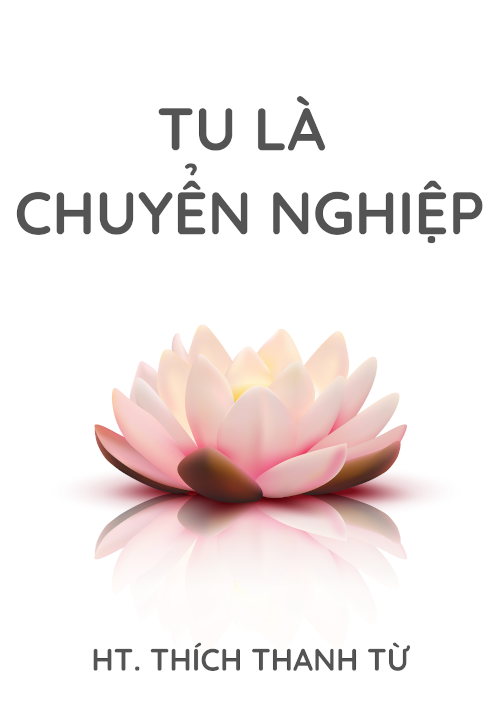
\includegraphics[width=4.29167in,height=\textheight]{images/cover_resized.png}

Tuyển tập 7 bài viết về Nghiệp trong Phật giáo của Hòa thượng Thích Thanh Từ:

\begin{itemize}
\tightlist
\item
  \href{https://phapduyen.github.io/tu-la-chuyen-nghiep/tu-la-phai-hien}{Tu là phải hiền}
\item
  \href{https://phapduyen.github.io/tu-la-chuyen-nghiep/nghiep-dan-di-trong-luan-hoi-luc-dao}{Nghiệp dẫn đi trong luân hồi lục đạo}
\item
  \href{https://phapduyen.github.io/tu-la-chuyen-nghiep/biet-nghiep-va-dong-nghiep}{Biệt nghiệp và đồng nghiệp}
\item
  \href{https://phapduyen.github.io/tu-la-chuyen-nghiep/chanh-bao-va-y-bao}{Chánh báo và y báo}
\item
  \href{https://phapduyen.github.io/tu-la-chuyen-nghiep/bo-tat-so-nhan-chung-sanh-so-qua}{Bồ Tát sợ nhân, chúng sanh sợ quả}
\item
  \href{https://phapduyen.github.io/tu-la-chuyen-nghiep/than-thong-va-nghiep-luc}{Thần thông và nghiệp lực}
\item
  \href{https://phapduyen.github.io/tu-la-chuyen-nghiep/tu-co-chuyen-duoc-nhan-qua-khong}{Tu có chuyển được nhân quả không?}
\end{itemize}

Download:

\begin{itemize}
\tightlist
\item
  \href{https://phapduyen.github.io/tu-la-chuyen-nghiep/tu-la-chuyen-nghiep.epub}{EPUB}
\item
  \href{https://phapduyen.github.io/tu-la-chuyen-nghiep/tu-la-chuyen-nghiep.pdf}{PDF}
\end{itemize}

Hoan nghênh chia sẻ, phổ biến!

\begin{center}\rule{0.5\linewidth}{0.5pt}\end{center}

Icons made by \href{https://www.flaticon.com/authors/vectors-market}{Vectors Market} from \href{https://www.flaticon.com}{www.flaticon.com}\\
\href{https://www.freepik.com/vectors/background}{Background vector created by macrovector\_official - www.freepik.com}

\hypertarget{tu-la-phai-hien}{%
\chapter*{Tu là phải hiền}\label{tu-la-phai-hien}}
\addcontentsline{toc}{chapter}{Tu là phải hiền}

Buổi nói chuyện hôm nay, tôi nhắm vào Quý Phật tử Phước Thái nhiều hơn là Quý Phật tử ở các nơi. Vậy quý vị hãy lắng nghe cho kỹ. Ở đây, tôi không giảng những đề tài cao siêu mà đặt những câu hỏi rất thực tế, rất thấp, quý vị hãy trả lời đúng như chỗ mình biết, để rồi tôi hướng dẫn cho quý vị tu hành.

- Quý vị đi chùa học đạo, có phải tu theo đạo Phật không?

- Thưa phải.

- Vậy người tu là hiền hay dữ?

- Dạ hiền.

- Người đi chùa, lạy Phật, ăn chay, tụng kinh, nếu có người xúc phạm đến thì nóng nảy la lối. Như vậy có hiền không?

- Dạ chưa hiền.

- À, chưa hiền tức là chưa tu. Vậy đi chùa tụng kinh mà chưa hiền, chưa gọi là người tu. Người tự nhận mình tu theo đạo Phật mà chưa hiền thì sao? Phải tu thế nào mới gọi là tu theo đạo Phật. Và làm thế nào để được hiền, quý vị biết không?

- Dạ chưa biết.

- Đây, tôi hướng dẫn cho quý vị để thành người hiền rất thực tế và dễ dàng. Theo tinh thần đạo Phật, tu là tu ở ba nghiệp: thân nghiệp, khẩu nghiệp và ý nghiệp.

Khi chưa biết tu, thân có khi làm lành, có lúc làm dữ; miệng có khi nói lời thiện, có lúc nói lời ác; ý có khi nghĩ tốt, có lúc nghĩ xấu.

Khi biết tu thì việc lành nên làm, việc dữ nên tránh. Lời thiện thì nói, lời ác thì chừa. Điều tốt thì nghĩ, điều xấu thì dừng. Người biết tu, thân không làm ác, miệng không nói ác, ý không nghĩ ác, đó là người hiền.

Tu chủ yếu không phải ăn chay nhiều. Vậy mà Phật tử cứ đua nhau ăn chay, cho ăn chay nhiều là tu, chứ không biết tu là chừa ba nghiệp ác. Nhân gian có câu ca dao để nhạo báng người ăn chay mà không hiền.

\begin{quote}
Sân si nghiệp chướng không chừa\\
Bo bo mà giữ tương dưa làm gì?
\end{quote}

Tham, sân, si là nghiệp chướng của thân, miệng và ý thì không chịu chừa bỏ, mà cứ đua nhau ăn chay, rồi cho đó là tu. Tu như vậy không đúng với chủ trương của đạo Phật. Tu là thân không làm ác, miệng không nói ác, ý không nghĩ ác.

Trong gia đình, nếu mọi người không biết tu thì cứ cãi và chửi bới gây phiền não cho nhau. Thậm chí, gây cãi không nguôi còn giận thì đánh đập. Đánh đập không thỏa mãn cơn giận thì tình nghĩa không còn. Mà tình nghĩa đã hết thì ly dị chia tay, gia đình đổ nát.

Nếu mọi người biết tu thì ý vừa khởi nghĩ ác liền biết xấu, chế ngự không dám nói lời nặng, không nói nặng thì đâu có cãi, không cãi thì làm gì có đánh đập, không đánh đập thì đâu có ly dị, gia đình thường an vui hạnh phúc.

Như vậy, nếu người biết tu thì ý không bao giờ nghĩ xấu cho ai, tâm không bực bội phiền não, lúc nào cũng vui vẻ an ổn. Nếu ý không nghĩ xấu thì miệng thân đâu có nói làm hung ác khiến cho người đau khổ. Mà không làm khổ người thì được người thương mến, người thương mến thì không hại, nếu có chuyện bất trắc thì được người giúp đỡ.

Khi đã biết tu thì thân, miệng, ý lúc nào cũng thiện. Ba nghiệp mà thiện thì tự thân được an vui, trong gia đình trên thuận dưới hòa, ngoài xã hội không gây xáo trộn sẽ được trật tự an bình. Như vậy, người biết tu, chẳng những chính bản thân mình được lợi ích, mà gia đình và xã hội cũng được lợi ích. Đó là người tu đúng theo lời Phật dạy.

Nếu chỉ biết ăn chay, tay lần tràng hạt, mỗi khi có ai xúc phạm đến thì la lối, chửi rủa không thua ai; người như thế không hiền, chưa phải là người tu. Do vậy, nên bị chế nhạo: \emph{``Ngoài miệng thì nam mô, trong bụng thì chứa một bồ dao găm''.}

Ngoài miệng thì niệm Phật lâm râm, nhưng trong tâm thì quá hung dữ. Thế nên, cho ăn chay nhiều, niệm Phật nhiều là tu mà không chịu chuyển thân, miệng, ý cho thiện thì làm trò cười cho thiên hạ. Vì vậy, khi nói tới tu, người Phật tử phải nhớ thân, miệng, ý phải thiện.

Phật dạy, tu một giờ, là được an vui hạnh phúc một giờ, tu một ngày là được an vui hạnh phúc một ngày, tu một năm là được an vui hạnh phúc một năm. Nhưng gần đây, có một số Phật tử nghĩ rằng ăn chay, đi chùa, làm công quả có phước nên ham đua nhau làm.

Ví dụ, trong gia đình, trung bình ăn chay một tháng bốn ngày. Vì nghe nói ăn chay có phước nhiều được khen, nên người vợ tăng thêm sáu ngày, rồi mười ngày\ldots{} Chồng con ăn theo không nổi nên có chuyện xào xáo trong gia đình. Rồi than trách rằng mình muốn tu, muốn tiến mà bị quỉ nó phá, nó ngăn không cho tu tiến. Người nghĩ nói như vậy có tu không? Tu mà ý khởi nghĩ ác, miệng chửi chồng con là quỉ. Như vậy, chưa phải là người Phật tử chân chính.

Người Phật tử chân chính không đặt nặng việc đi chùa thường xuyên, tụng kinh giỏi, ăn chay nhiều, mà phải biết tu ba nghiệp thân, khẩu, ý cho thiện. Tức là chuyển ba nghiệp ác thành ba nghiệp thiện. Đi chùa, niệm Phật, ăn chay là phải nhớ từng hành động, từng lời nói, từng ý nghĩ luôn luôn phải thiện. Như vậy, có lúc nào là không tu.

Chẳng hạn, thân cuốc cỏ, xưa thấy rắn thì lấy cuốc đập chết, nay thấy rắn tránh không đập, đó là chuyển nghiệp thân ác thành thiện. Xưa khi tiếp xúc với bạn bè, họ nói lời hung dữ làm mình tức giận, bèn nói nặng lời cho bõ ghét. Nhưng nay nhớ mình là người tu, không được lớn tiếng gây cãi, nên im lặng mà nhẫn nhịn. Đó là chuyển nghiệp khẩu ác thành thiện. Lúc ngồi một mình, vừa khởi nghĩ xấu về người liền hổ thẹn, dừng không nghĩ nữa. Đó là chuyển nghiệp ý ác thành thiện.

Tu như vậy, đâu có đợi vô chùa tụng kinh lạy Phật mới tu, mà giờ nào, ở đâu tu cũng được. Thế mới đúng ý nghĩa tu của đạo Phật. Nếu hiểu và tu như vậy, thì lo gì mai kia không được về cõi Phật. Trong kinh có câu:

\begin{quote}
Tam nghiệp hằng thanh tịnh\\
Đồng Phật vãng Tây phương
\end{quote}

Ba nghiệp mà hằng trong sạch thì đồng với Phật, về cõi Phật. Nếu không bỏ ba nghiệp ác mà cố niệm Phật nhiều, cầu Phật A-Di-Dà rước về Cực Lạc, cũng không được rước về. Vì ba nghiệp còn ác thì về đó cứ gây cãi, đánh đập hoài biến cõi Cực Lạc thành cõi Ta Bà khổ hay sao?

Vậy, tu cốt là chuyển ba nghiệp ác thành ba nghiệp thiện là bước đầu, tụng kinh niệm Phật là bước kế tiếp. Bước đầu là nền tảng mà không thực hiện trước, lại đi bước thứ hai, giống như cất nhà lầu mà không xây nền móng, nhất định cái nhà sẽ đổ không thành.

Lại cũng có nhiều Phật tử đi chùa lâu năm, ăn chay, niệm Phật, nếu con cháu có làm gì phật ý thì mắng chửi không tiếc lời, khiến cho con cháu buồn không thương mến. Rồi viện cớ là chỉ hiền với người ngoài thôi, đối với con cháu trong nhà phải khó, phải dữ nó mới sợ. Người Phật tử nói vậy là không đúng. Tu là phải hiền, hiền với tất cả mọi người, từ trong nhà cho đến ngoài xã hội. Giả sử con cháu có làm bậy, làm sai, thì nên ôn tồn nhỏ nhẹ khuyên dạy con cháu. Đừng nên chửi bới la rầy, vì lúc nóng giận không kiểm soát được ý nghĩ, lời nói, sẽ nói bậy. Mà nói bậy thì mất uy tín với con cháu.

Kinh Phật ví dụ một Trưởng giả có tất cả bốn bà vợ. Người thứ nhất rất trung thành với ông, thế mà suốt ngày ông không nghĩ tới. Người vợ thứ hai được ông lưu ý chút ít. Người vợ thứ ba được ông nhắc nhở liền miệng. Người vợ thứ tư thì ông ở đâu bà có mặt ở nơi đó, không rời một gang tấc. Một hôm ông đau nặng sắp chết, hỏi cả bốn người vợ:

- Tôi sắp chết, trong bốn bà có ai nguyện chết theo tôi không?

Vợ thứ tư lên tiếng trước:

- Bình thường ông ở đâu thì có mặt tôi ở đó. Bây giờ ông chết, tôi xin đưa ông tới cửa.

Vợ thứ ba lên tiếng tiếp:

- Bình thường tôi được ông lưu ý nhắc nhở liền miệng. Bây giờ ông chết, tôi xin đưa ông tới cổng.

Vợ thứ hai nói:

- Bình thường tôi cũng được ông nhắc nhở. Bây giờ ông chết, tôi xin đưa ông tới mộ.

Vợ thứ nhất nói:

- Bình thường tuy ông không nghĩ tới, nhưng bây giờ ông chết, tôi nguyện chết theo ông.

Quý vị thấy ông Trưởng giả quá bất công và bội bạc. Người thương mình, trung thành với mình thì lơ là không nghĩ đến. Người thương ít thì luôn luôn theo dõi không rời. Ông Trưởng giả bất công bội bạc này, Phật dụ cho mỗi người chúng ta.

Người vợ thứ tư, Phật dụ cho tiền bạc. Chúng ta ở nhà hay đi đâu đều có tiền trong túi không thể thiếu nó. Nhưng khi chúng ta chết thì nó nằm trong tủ hoặc ở nơi rương thuộc phạm vi trong nhà. Vì vậy mà nói đưa tới cửa.

Người vợ thứ ba dụ cho của cải sự nghiệp, nhà cửa. Nó nằm ở trong phạm vi vòng rào nhà, nên nói đưa tới cổng.

Người vợ thứ hai dụ cho công danh, chức tước. Khi đưa quan tài người chết tới huyệt thì đọc điếu văn kể công trạng rồi mới hạ huyệt chôn cất, nên nói đưa tới mộ.

Người vợ thứ nhất dụ cho nghiệp lành hay nghiệp dữ theo mình như hình với bóng. Có mình ở đâu thì có nó ở đó không rời nhau, nên mới tình nguyện chết theo.

Tác động của thân, khẩu, ý lặp tới lặp lui nhiều lần gọi là nghiệp. Người dạy học hằng ngày thì gọi là nghề giáo hay nghiệp giáo. Người cùng làm một việc thì gọi là bạn đồng nghiệp. Có người là có nghiệp. Người nghiệp không rời nhau.

Giả sử như ông thầy giáo đi đường có mang theo một số tiền của. Bất thần ông bị tai nạn, bao nhiêu tiền ông mang theo bị mất hết. Nhưng nghiệp dạy học vẫn còn không mất, về nhà vẫn đến trường dạy học trò. Như vậy, tiền của và tài sản là cái ngoài mình nên bị mất dễ dàng, không thể giữ được mãi mãi. Còn nghiệp là cái không ngoài mình nên chẳng bao giờ mất. Thế mà trong cuộc sống hằng ngày, mọi người đều nghĩ làm sao cho có tiền, làm sao cho có của. Nếu có tiền, có của rồi thì muốn có địa vị, danh vọng. Trong ba thứ đó, nghĩ tới tiền nhiều nhất, rồi tới của cải, danh vọng. Khi chết, thì tiền của từ giã mình trước nhất, tức là khi chết nó ở lại chứ không theo mình.

Trong đời này không ai là (người) không chết. Hoặc chết sớm, hoặc chết muộn. Khi chết thì không ai đem được tiền của theo, chỉ có nghiệp lành hay nghiệp dữ theo mà thôi. Thế nên, nếu là người Phật tử khôn ngoan sáng suốt, dù có làm ra nhiều tiền của mà làm ác thì nhất định không làm. Vì khi chết không cứu được tội khổ mà phải để lại tất cả, chỉ có một mình mình chịu quả báo khổ đau. Nghĩ và nói ác mà đem lại lợi lộc cho mình thì cũng không nói. Như thế không bị tiền tài sai sử tạo nghiệp ác.

Ngày nay không gây tạo tội lỗi, không bị người chê trách, mai kia chết đi cũng nhẹ nhàng thảnh thơi. Ca dao có câu:

\begin{quote}
Bởi chừng kiếp trước khéo tu,\\
Ngày nay con cái võng dù nghênh ngang
\end{quote}

Do kiếp trước khéo tu nên ngày nay con cháu mới sang trọng. Nếu hiện tại không chịu tu thì con cháu về sau khổ. Để thấy chúng ta tu là tạo cho cuộc sống hiện tại an vui, ngày mai lại càng an vui tốt đẹp hơn. Vậy, biết tu là thường nhớ tới nghiệp, để tránh nghiệp ác, làm nghiệp lành, hơn là nhớ tới tiền của, vật chất. Tuy trong cuộc sống, chúng ta phải làm ra tiền mới sống được, nhưng phải làm cho công bằng lương thiện. Mình an vui, người không khổ, hiện tại mình hạnh phúc, mai sau cũng an lành. Vậy, tu không phải là mong cầu cái gì cao siêu huyền bí, mà ngay trong thực tế thường làm lợi mình, lợi người một cách cụ thể, không mơ hồ viễn vông.

Đạo Phật chủ trương tu là để giải thoát, song nói giải thoát có vẻ xa vời quá! Nhưng nếu thực tế, thân chúng ta không làm ác là giải thoát được cái khổ nghiệp ác của thân. Vì nếu cướp của giết người thì bị cái khổ đánh đập tù tội. Bây giờ không tạo nghiệp ác ấy thì thân được lành mạnh tự do, đó là giải thoát nghiệp ác của thân.

Nếu miệng không nói lời hung dữ ác độc thì giải thoát được nghiệp ác của miệng. Ý không nghĩ ác thì giải thoát được tâm niệm xấu xa, buồn ghét người khác. Tuy không hoàn toàn giải thoát nhưng có giải thoát từng phần. Tu ít thì giải thoát ít, tu nhiều thì giải thoát nhiều, có tu là có bớt khổ. Chẳng những bớt khổ trong đời này mà trong đời sau còn được an vui nữa. Nên người biết tu không sợ chết. Vì ai cũng phải chết, và biết rằng mình không tạo nghiệp ác thường tạo nghiệp lành, sau khi chết sẽ an vui chớ không khổ. Tuy nhiên, đừng vì muốn giải thoát mà liều chết sớm để được khỏe được sướng thì không đúng với tinh thần giải thoát của đạo Phật.

Thông thường thì người đời tham sống sợ chết, nên nghe nói chết thì rất sợ. Nhưng người biết tu thì ngay cuộc sống hiện tại lúc nào cũng an vui, khi chết đến thì bình thản không loạn động, nên không muốn chết sớm mà cũng không sợ chết. Vì vậy mà Phật tổ mới dạy chúng ta tu, tu là nguồn cội hạnh phúc, hết phiền não, hết khổ đau.

Kể từ ngày nay, quý Phật tử ở gần thiền viện, mỗi tháng hai lần vào ngày rằm và ba mươi nên đi chùa sám hối và nghe quý thầy giảng để biết phương hướng mà tu tập. Nghe một lần tuy biết đó, nhưng vì cái bệnh chúng sanh hay quên, nên mỗi tháng phải đi hai lần, nhờ các thầy nhắc nhở, luôn ghi nhớ mới tinh tấn mà tu hành.

\hypertarget{nghiep-dan-di-trong-luan-hoi-luc-dao}{%
\chapter*{Nghiệp dẫn đi trong luân hồi lục đạo}\label{nghiep-dan-di-trong-luan-hoi-luc-dao}}
\addcontentsline{toc}{chapter}{Nghiệp dẫn đi trong luân hồi lục đạo}

Giáo lý của nhà Phật cốt yếu dạy cho con người tu để giải thoát luân hồi sanh tử. Tuy nhiên, tùy theo sức huân tu cao thấp mà giải thoát cũng có nhiều từng bậc. Đại lược chúng ta có thể chia làm hai bậc là: Từng phần giải thoát và toàn phần giải thoát.

Từng phần giải thoát là bậc thứ nhất, tu mà còn luân hồi sanh tử, nhưng biết chọn lựa phước lành để đi trong đường tốt hưởng phước báo. Những loại chúng sanh đi trong các đường địa ngục, ngạ quỉ, súc sanh, A-tu-la đều không biết chọn nghiệp lành nên đi vào con đường ác, chịu quả báo khổ đau. Và ngay như loài người có biết chọn nghiệp thiện, lại cũng có người không biết chọn nên tạo lắm nghiệp ác. Vì vậy mà chịu không biết bao nhiêu thứ khổ đau.

Thế nên, khi còn ở trong lục đạo luân hồi, sau khi bỏ thân này, muốn cho đời sống của thân sau được an vui hạnh phúc thì ngay hiện tại phải biết chọn lựa nghiệp lành để làm và để tránh ba nghiệp ác, đó là gốc của sự tu hành.

Nghiệp là động lực dẫn chúng ta đi trong luân hồi sanh tử, nên rất hệ trọng đối với sự tu hành. Vậy nghiệp là gì? Nghiệp được dịch từ chữ Phạn Karma nghĩa là hành động lặp đi lặp lại nhiều lần thành thói quen. Thói quen đó gọi là nghiệp.

Ví dụ giáo viên dạy học, dạy từ năm này qua năm khác, được gọi là nghề giáo và những người làm cùng nghề thì gọi là bạn đồng nghiệp.

Nghiệp là việc làm của chính mình, mình làm chủ và tạo tác thành thói quen, rồi cũng chính mình thừa nhận hậu quả do nó đưa tới. Kinh Phật dạy: \emph{``Chúng sanh làm chủ tạo nghiệp và thừa kế cái nghiệp do chính mình đã tạo''}. Không do ai khác ngoài mình.

Chúng ta từ thuở sơ sinh cho tới chín, mười tuổi đâu có ai mắc bệnh ghiền rượu, ghiền trầu hay ghiền thuốc\ldots{} Thế mà từ 15, 16 tuổi cho tới già, do sự tập tành thành thói quen, người thì ghiền rượu, người thì ghiền thuốc, kẻ thì ghiền á phiện\ldots{}

Đứa trẻ 15, 16 tuổi thấy người lớn cầm thuốc hút nhả khói phì phà tưởng đó là oai là sang, nên bắt chước hút, thành thói quen rồi ghiền thuốc. Lúc mới tập hút thì mình làm chủ, thích hút thì hút, không thích hút thì thôi. Nhưng hút nhiều lần dần dần thành thói quen, thiếu thuốc thì khó chịu, ngáp, buồn, phải đi mua về hút. Vậy khi đã ghiền rồi thì không còn làm chủ nữa mà nó làm chủ ngược lại mình, sai sử mình làm theo thói quen ưa thích đó. Vậy, nghiệp là cái chúng ta tự tạo, chúng ta làm chủ tạo thành thói quen. Khi thói quen thuần thục thì nó làm chủ dẫn dắt sai sử chúng ta.

Nếu ta tập thói quen làm việc thiện thì được dẫn dắt tiếp tục làm việc thiện. Nếu chúng ta tập thói quen làm việc bất thiện thì bị dẫn dắt tiếp tục làm việc bất thiện.

Chẳng hạn, người mỗi chiều đi chùa tụng kinh lâu ngày thành thói quen. Một hôm, tới giờ tụng kinh không đi cảm thấy thiếu, thấy buồn, có một động lực thôi thúc bắt phải đi chùa tụng kinh.

Còn người khác, mỗi chiều đi quán uống rượu, lâu ngày thành thói quen nên ghiền. Tới cữ đi uống rượu, không đi thì cảm thấy bức rức khó chịu, ngáp dài, có một ma lực thôi thúc sai khiến tới quán rượu để uống rượu.

Người đi chùa tụng kinh tập thành thói quen đó là nghiệp thiện, đưa tới sự an vui lợi ích cho bản thân mình. Người đi quán uống rượu tập thành thói quen là nghiệp ác, đưa tới nghèo thiếu, bệnh hoạn, kém trí tuệ.

Vậy, nghiệp phát xuất từ đâu? Nếu thân tạo tác thiện đó là nghiệp thiện của thân, thân tạo tác ác đó là nghiệp ác của thân. Miệng nói điều lành là nghiệp thiện của miệng, miệng nói lời hung dữ là nghiệp ác của miệng. Ý nghĩ tốt là nghiệp thiện của ý, ý nghĩ xấu là nghiệp ác của ý. Đó là nghiệp phát xuất từ thân, khẩu, ý.

Như vậy, tạo nghiệp chủ động là mình. Nếu muốn luân hồi chỗ tốt, cho thân lành mạnh tốt đẹp, được sống an vui hạnh phúc thì hiện tại phải biết tạo nghiệp thiện. Nếu ngược lại, tạo nghiệp ác thì luân hồi đến cõi xấu, thọ thân xấu, sống đời đầy đau khổ. Do mình chủ động trọn vẹn, chớ không do ai khác. Ngay trời Phật cũng không dự phần trong đó.

Như vậy, chúng ta là chủ chọn lấy hướng đi cho chúng ta mai sau. Nếu khôn ngoan đã chọn cho mình một hướng đi tốt đẹp thì cứ theo hướng đó mà đi, chớ có thay đổi.

Cũng như các học sinh sau khi đã chọn nghề và tốt nghiệp ra trường, phải theo cái nghề mình đã chọn mà sống. Sướng hay khổ tùy theo cái nghề của mình chọn.

Vậy, chúng ta tu là phải làm sao? Có nhiều Phật tử than vì bệnh tật, vì nghèo khổ không thể tu. Người than như vậy là chưa biết tu, vì họ tưởng phải đi chùa nhiều, tụng kinh giỏi mới là tu. Như đã nói, tu là chuyển nghiệp ác thành nghiệp thiện, mà nghiệp thì phát xuất từ thân, khẩu, ý.

Giả sử như người buôn bán, nếu tráo hàng thật ra hàng giả, hoặc cân đo thiếu, hoặc bán người trả giá không đúng, nổi giận la chửi, đó là thân miệng tạo nghiệp ác, không biết tu.

Nếu buôn bán với mức lời vừa phải, hàng thật nói là hàng thật, hàng giả nói là hàng giả, cân đo đúng, khách trả đúng giá thì vui vẻ bán, khách trả không đúng giá tuy không bán vẫn vui cười, không tức giận mắng chửi.

Hoặc đi đường gặp người già yếu nhường lối đi, nhường chỗ ngồi, đưa qua đưòng, đưa qua cầu, bưng xách nặng dùm người\ldots{} đó là thân khẩu thiện, biết tu. Tu trong công ăn việc làm, tu ngoài đường, tu ngoài chợ.

Ở trong nhà, đối với người thân cũng phải giữ thân miệng luôn lành. Làm cha mẹ giữ đúng tư cách của cha mẹ, con cái có lỗi lầm phải từ tốn răn dạy, hướng dẫn phù hợp với đạo lý cho con nên người, đó là tu. Nếu ỷ quyền cha mẹ, khi con làm không vừa ý, tay đánh đập, miệng la hét, chửi rủa, đó là không biết tu. Phận làm con đối với cha mẹ phải biết thương kính, chăm lo việc ăn mặc thuốc thang cho cha mẹ, đừng để cha mẹ buồn tủi lúc tuổi già. Nếu cha mẹ có sanh tật khó khăn thì nên an ủi khuyên lơn hơn là hờn trách chế diễu. Đó là chuyển nghiệp thân, nghiệp khẩu luôn lành.

Về ý nghiệp có phần vi tế hơn, với người biết tu cũng chuyển được nghiệp ác thành nghiệp thiện. Nếu đang ngồi chơi hay đi, hoặc làm việc, khởi nghĩ buồn giận người, biết đó là ác ý liền dừng không nghĩ, mà khởi nghĩ thương người nghèo khó, quý kính bậc hiền đức, tìm cách giúp đỡ người khốn khổ\ldots{} Đó là chuyển nghiệp ý ác thành ý thiện.

Nếu cho rằng đi chùa hay tụng kinh mới là tu, thì tu quá ít. Rồi bệnh nào tật ấy vẫn còn nguyên. Tham, sân, si, ích kỷ vẫn không chừa, tu như thế hiện tại tự mình không lợi ích và cũng không đem được an hòa cho mọi người chung quanh, mai sau bị nghiệp lôi vào đường ác là địa ngục, ngạ quỉ, súc sanh.

Thế nên, Phật dạy trong tất cả ngày giờ của mọi sinh hoạt đều phải tu mới chuyển được ba nghiệp trọn lành. Ba nghiệp lành rồi, ngay đời hiện tại tự mình không phiền não, lúc nào cũng nhẹ nhàng an vui. Trong gia đình mọi người không thắc mắc rày rà, trên thuận dưới hòa, đầm ấm hạnh phúc. Ngoài xã hội được an bình, không loạn ly. Tu như thế mới thật là tu. Đừng vì muốn được đi chùa thường xuyên, muốn được tụng kinh nhiều mà phế bỏ cả việc nhà. Thân, miệng, ý không chuyển cho lành, về nhà thì thắc mắc, gây cãi hết người này tới người nọ làm cho gia đình xào xáo. Đối với người ngoài xã hội thì không nhịn một lời, không nhượng một bước. Đi chùa tụng kinh như thế là chưa thật tu.

Có một bà cụ Nhật Bản lần chuỗi niệm Phật rất giỏi. Khi lần chuỗi niệm Phật thì rất chăm chỉ, nhưng khi dừng niệm Phật thì rầy rà con cháu inh ỏi. Con trai bà thấy bà tu như thế nó buồn và nói:

- Má à, má tu má cứ lo niệm Phật đi, sao má cứ rầy rà hoài khiến xao lãng làm sao Phật chứng cho má?

Bà nói:

- Khi nào tao niệm Phật thì Phật thông cảm cho tao, còn khi nào tao rầy tụi bây thì tụi bây biết cho tao.

Bà chia làm hai phần, phần niệm Phật thì tu với Phật, phần rầy la thì dành cho con cháu! Người thật tu là vừa tu với Phật cũng vừa tu với thế gian, tu như thế mới trọn vẹn.

Có người ngoại đạo đến hỏi Phật:

- Thưa ngài Cồ Đàm \emph{(họ Gautama, tên Siddhartha dòng Shakya, của Đức Phật Thích-Ca)}, cái gì định đặt cho con người, sinh ra kẻ thì nghèo nàn khổ sở, người thì giàu sang sung sướng, kẻ thì sống lâu, người thì chết yểu, kẻ thì yếu đau, người thì khỏe mạnh, kẻ thì ngu dốt, người thì thông minh?

Phật trả lời:

- Tất cả sự sai biệt giữa con người và con người là do nghiệp mà họ đã tạo định đặt ra, nên có người ưu, kẻ liệt.

- Do tạo nghiệp gì khiến cho con người sống lâu và do tạo nghiệp gì khiến cho người chết yểu?

- Người không tạo nghiệp sát hại chúng sanh thì được thọ mạng lâu dài. Người tạo nghiệp sát, đoản mạng sống của chúng sanh nên thọ mạng yểu.

- Do tạo nghiệp gì thân người được khoẻ mạnh và do tạo nghiệp gì mà thân hay yếu đau bệnh tật?

- Do nghiệp ác làm cho người đau khổ nên thọ thân hay bệnh tật đau yếu. Và do nghiệp lành an ủi giúp đỡ người qua những tai nạn khốn khó nên được thọ thân khỏe mạnh vui tươi.

- Do tạo nghiệp gì mà sinh thân trong gia đình giàu sang sung sướng và do tạo nghiệp gì mà sinh thân trong gia đình nghèo khó khốn khổ?

- Do đời trước biết làm lành, biết bố thí cúng dường, biết giúp đỡ người nghèo khó bệnh tật, nên đời này được sinh ra trong cảnh giàu sang sung sướng. Người ở đời trước không biết bố thí cúng dường, không biết giúp đỡ người nghèo khó, lại còn tham lam rút rỉa của người nên đời này sanh thân trong cảnh nghèo đói thiếu thốn.

- Do nghiệp gì người sanh ra được thông minh sáng suốt và do nghiệp gì người sanh ra lại ngu dốt tối tăm?

- Người đời trước do siêng năng học hỏi tìm hiểu chân lý, ưa thích giúp người được học hỏi hiểu biết nên đời này được thông minh. Người ở đời trước do lười biếng học, không chịu tìm hiểu chân lý, cản ngăn sự học hỏi của người nên đời này bị tối tăm mê mờ.

Vậy, tất cả quả tốt hay xấu mà chúng ta đang thọ hiện nay, gốc là từ cái nhân chúng ta gây thuở trước, chứ không phải bỗng dưng mà có. Khi đã biết như thế, chúng ta muốn ngày mai được tốt đẹp an vui hay bị đau khổ, thì ngay bây giờ chúng ta phải chuẩn bị.

Nếu chuẩn bị bằng nghiệp lành thì sẽ được đến cõi lành và được an vui hạnh phúc. Nếu chuẩn bị bằng nghiệp ác thì sẽ đi vào đường dữ và bị khổ đau.

Có người nêu nghi vấn: Hiện tại thân này hành động tạo nghiệp thiện hay ác, mai kia thân hoại rồi hành động cũng mất, vậy nghiệp còn hay mất? Đa số người không tin nhân quả, họ nghĩ rằng sau khi thân hoại hành động cũng không còn thì nghiệp cũng mất.

Trong kinh Phật thường nói nghiệp theo mình như bóng với hình vậy. Đời quá khứ, đời hiện tại, đời vị lai có sự liên hệ tùy theo nghiệp của mỗi người.

Ví dụ, có hai người khách qua sông, một người chuyên nghề giáo, một người chuyên nghề thương mãi. Khi đi đường người thương mãi đem theo nhiều vàng bạc của cải, nhà giáo chỉ mang theo một cặp sách vở và chút ít tiền lộ phí. Thuyền qua giữa sông bất thần gặp sóng làm chìm. Khi thuyền chìm, mạnh ai nấy lo, lội vào bờ để thoát chết. Lên đến bờ thì tất cả của cải, tiền bạc của nhà thương mãi không còn, cặp giấy tờ, tiền lộ phí của nhà giáo cũng mất. Cả hai đều trắng tay, nhưng kiến thức giáo dục của nhà giáo không mất, kiến thức mua bán của nhà thương mãi cũng không mất. Kiến thức là cái chuyên môn sở trường của con người không mất, tức là nghề nghiệp không mất.

Như vậy, để thấy, qua những cuộc biến đổi, tất cả những cái có hình tướng ngoài mình thì mất. Nên khi thân này có hoại đi, nghiệp thức không ngoài mình nên không mất. Của cải tài sản thế gian, chúng ta tạo sắm nhiều thế mấy, khi chết rồi tất cả đều phải để lại, không đem theo được một món nào, chỉ có mang theo nghiệp mà thôi. Đó là một lẽ thật. Thế mà, có nhiều người không hiểu không tin, rồi mê tín dán nhà lầu xe hơi, mua giấy tiền vàng bạc đốt để đem theo cho cha mẹ chồng con chết xài.

Có người vội hỏi:

- Con cháu vì thương cha mẹ, sau khi cha mẹ chết họ dán nhà, xe, mua giấy tiền vàng thật nhiều đem đốt và cầu nguyện cho cha mẹ được hưởng. Như vậy, cha mẹ có được hưởng không?

- Nếu con cháu đốt giấy tiền vàng bạc rồi cầu nguyện cho cha mẹ lãnh, tôi e rằng ở tù chớ chẳng được hưởng. Tại sao? Vì mang bạc giả xuống diêm vương xài là bất hợp pháp. Nếu đốt nhà lầu xe hơi giấy, cầu cho thân nhân mình lãnh về ở và đi, tôi cho rằng nếu ai làm như vậy là hại thân nhân của mình. Vì nếu họ nhận được thì họ có nhà lầu để ở, có xe hơi để đi, có tiền bạc để xài, đủ tiện nghi quá thì họ sẽ ở mãi cõi âm, không đi đầu thai. Đó là trường hợp thân nhân của mình trong sanh tiền có chút phước lành.

Còn nếu là kẻ có tội thì chết đọa địa ngục bị giam nhốt hành hạ làm sao mà nhận lãnh tiền bạc nhà xe để xài? Đó là chưa nói đến nhà xe tiền bạc bị đốt thành tro thì dùng làm sao được? Thật là vô lý!

Như vậy, để thấy chính nghiệp lành hay dữ mà mình tạo ra nó dẫn mình đi thọ thân trong cảnh giới sướng hay khổ. Tất cả việc làm bên ngoài của người thân vì thương muốn giúp mình khó mà giúp được, mình làm mình phải chịu, người khác không thể thế được.

Lại có người nêu câu hỏi:

- Tại sao có nhiều người làm ác mà họ sống phây phây? Có nhiều người rất hiền lành, làm phước, làm nghĩa mà lại gặp nhiều hoạn nạn. Như vậy là luật nhân quả bất công sao? Lại có nhiều người không làm ác, vừa làm ác thọ quả báo liền, hoặc vừa làm thiện thì thọ quả báo lành liền. Như vậy là sao?

Trong kinh Phật có dạy: Nếu tạo nghiệp thiện được phước báo lành, tạo nghiệp ác bị quả báo khổ thì Phật chấp nhận. Nếu nói rằng làm nghiệp thiện sau khi chết sẽ sanh về cõi Trời, làm nghiệp ác sau khi chết sẽ đọa xuống địa ngục liền, điều đó Phật không chấp nhận.

Tại sao nói làm ác chịu chịu quả báo ác, làm thiện được quả báo thiện, thì Phật chấp nhận. Mà nói tạo nghiệp ác sau khi chết đọa địa ngục, làm lành sau khi chết về cõi Trời thì Phật không chấp nhận?

Về thuyết nghiệp, Phật có nói cận tử nghiệp và tích luỹ nghiệp. Tích lũy nghiệp chứa từ nhiều kiếp đến giờ. Cận tử nghiệp là nghiệp mới tạo tác lúc sắp chết. Cận tử nghiệp và tích lũy nghiệp có ảnh hưởng chi phối nhau mà quyết định đưa người chết đến cõi lành hay cõi dữ.

Ví dụ, có người tích lũy nghiệp lành từ xưa đến nay, bất thần họ mê muội có người xúi dục họ làm điều ác. Làm điều ác này đáng lý phải đọa địa ngục, nhưng vì tích lũy nghiệp lành họ còn nhiều nên chưa đọa địa ngục liền.

Lại cũng có người làm nhiều điều ác, đáng lý phải đọa địa ngục, nhưng gần chết họ làm lành, tâm họ luôn nghĩ tưởng đến điều lành nên không đọa địa ngục. Thế nên, nói làm ác khi chết nhất định đọa địa ngục, làm thiện lên thiên đàng, thì không đúng hẳn. Vì tuy họ có làm ác, nhưng lúc gần chết, cận tử nghiệp thiện họ quá mạnh có thể đưa họ đến cõi thiện.

Còn người tuy làm nhiều điều thiện, nhưng khi gần chết họ nổi sân quá hung dữ. Lúc đó, cận tử nghiệp ác có thể đưa họ đến các đường xấu. Thế nên, không phải chỉ tu khi sắp chết, hoặc chỉ tu ở giai đoạn thân còn mạnh khỏe mà phải luôn luôn giữ thân, khẩu, ý lành, từ lúc còn trẻ trung mạnh khỏe cho đến chung cuộc của kiếp người.

Xưa có Maha Nam, con của Cam Lộ Phạm Vương, em nhà chú của Đức Phật. Maha Nam tu cư sĩ, giữ năm giới, tu thập thiện, thọ bát quan trai\ldots{} Một hôm hỏi Phật rằng:

- Bạch Thế Tôn, bình thường con tu giữ năm giới, thọ bát quan trai, tu thập thiện. Giả sử con chết bất đắc kỳ tử bởi một tai nạn xảy ra, sau khi chết con sẽ đi về đâu?

Phật trả lời bằng một ví dụ:

- Có một cây mọc từ đất lên, thân và cành cây nghiêng về một bên. Vậy khi cưa, thân ngã về bên nào?

Maha Nam đáp:

- Cây ngã về phía mà nó đang nghiêng.

Phật dạy tiếp:

- Cũng vậy, bình thường ông hay làm điều lành, khi chết tuy bị khủng hoảng, nhưng nghiệp thiện tích lũy nhiều sẽ hướng ông đến chỗ lành. Không sao, đừng sợ.

Vậy, chủ yếu của việc tu hành, chẳng những tạo nghiệp lành trong lúc còn mạnh khỏe mà lúc gần chết tâm niệm cũng phải lành thì mới bảo đảm đi đến cõi lành. Và bình thường tạo nghiệp lành, mà lúc gần chết tạo nghiệp dữ thì chưa bảo đảm đi đến cõi lành. Và bình thường nếu lỡ làm ác, lúc gần chết tâm niệm lành thì cũng chuyển được phần nào nghiệp dữ, vì nghiệp không cố định.

Để kết thúc buổi nói chuyện hôm nay, tôi nhắc lại câu chuyện Lý Bạch đời Đường ở Trung Hoa. Ông là một nhà thơ nổi tiếng, nghe danh Thiền Sư Ô Sào là một cao tăng đắc đạo mới tìm tới tham vấn. Tới nơi, thấy Thiền Sư Ô Sào ngồi trên cháng ba của một cây cổ thụ. Chỗ ngài ở giống như một ổ quạ nên người đời gọi Ngài là Thiền Sư Ô Sào. Ông đứng dưới đất nhìn lên hỏi:

- Bạch Hòa Thượng, Xin Hòa Thượng dạy cho tôi một phương pháp tu ngắn và gọn để tôi có thể tu được.

Thiền Sư Ô Sào ở trên nói xuống:

\begin{quote}
Chư ác mạc tác\\
Chúng thiện phụng hành\\
Tự tịnh ká ý\\
Thị chư Phật giáo
\end{quote}

Ông hãy về tu đi!

Lý Bạch nghe qua, cười và nói:

- Hòa Thượng nói bài kệ đó con nít tám tuổi cũng thuộc, vậy Hòa Thượng đem dạy tôi để làm gì?

Thiền Sư Ô Sào nói:

- Phải, con nít tám tuổi cũng thuộc nhưng ông già tám mươi tuổi làm cũng chưa xong.

\emph{``Chư ác mạc tác''} là tất cả nghiệp ác chớ có làm.

\emph{``Chúng thiện phụng hành''} là vâng làm tất cả các nghiệp lành.

\emph{``Tự tịnh ká ý''} là khéo lóng lặng tâm cho thanh tịnh.

\emph{``Thị chư Phật giáo''} đó là lời dạy của chư Phật.

Tu cốt là bỏ nghiệp ác của thân, khẩu, ý và chuyển thành nghiệp lành. Bài kệ trên vừa nghe qua là dễ nhớ và dường như thấy dễ làm. Song, đi vào kinh nghiệm tu hành thì không đơn giản và dễ dàng vì tình thức mênh mang, chủng tử tập khí sâu dày, vừa bỏ được thói xấu này để phát huy điều tốt nọ, thì lại có dư tập dở khác đang ngủ ngầm hội đủ duyên nó trổi dậy lại phải điều phục nữa. Và cứ thế làm mãi cho đến chung cuộc của kiếp người, có khi chưa xong, tâm vẫn còn lao xao, lộn xộn.

Thế nên, người biết hướng thiện luôn luôn phải xoay lại mình để lo tu tập, ở trong mọi hoàn cảnh, trong mọi trường hợp. Người rỗi rảnh hay bận rộn, giàu sang hay nghèo hèn ai cũng tu được. Điều tiên quyết là dừng nghiệp ác, rồi tùy theo hoàn cảnh: người nghèo thì ra công sức giúp đỡ, kẻ giàu thì ra tiền của bố thí. Ai ai cũng biết tu thì tự mình được an vui, gia đình được hạnh phúc, xã hội được an bình. Tu chính là nền tảng vững chắc để xây dựng cuộc đời hiện tại được tươi đẹp và tạo cơ hội cho đời sau càng được an vui, sáng suốt hơn.

Vậy, từ đây về sau trọn đời, quí Phật tử cố gắng tránh tất cả các điều ác, làm tất cả các nghiệp lành. Làm đó là làm cho chính mình chớ không phải làm cho ai khác. Đạo Phật được coi là đạo cứu khổ ban vui. Mà cứu khổ ban vui là chỉ cho mọi người con đường nào đi đến khổ đau và con đường nào đi đến an lạc. Khi biết con đường đưa tới an lạc thì cố gắng đi, đó là đạo Phật cứu khổ ban vui cho quý vị. Còn nếu quý vị biết con đường thiện đưa tới an lạc, con đường ác đưa tới khổ đau mà cứ đi con đường đau khổ thì đó là tại quý vị không biết chọn đường đi, khổ là do mình chớ không do ai khác. Vì Phật đã vạch lối chỉ đường rất rõ ràng, nếu chọn và thực hành đúng lời Phật dạy thì được an vui, lợi ích, ngược lại thì khổ đau. Đó là then chốt mà quý vị phải biết rõ và nắm vững để tu hành.

\hypertarget{biet-nghiep-va-dong-nghiep}{%
\chapter*{Biệt nghiệp và đồng nghiệp}\label{biet-nghiep-va-dong-nghiep}}
\addcontentsline{toc}{chapter}{Biệt nghiệp và đồng nghiệp}

Nghiệp là thói quen huân tập tạo thành sức mạnh chi phối tất cả mọi sinh hoạt trong cuộc sống của con người từ khi mở mắt chào đời cho đến khi nhắm mắt và những đời kế tiếp. Nếu người Phật tử tu mà không hiểu rõ về nghiệp thì khó mà ứng dụng tu hành để tới chỗ an lạc. Chữ nghiệp trong nhà Phật không có nghĩa một chiều, hễ nói nghiệp thì phải là điều xấu, điều ác. Kỳ thật, nghiệp cũng có xấu và cũng có tốt, nghiệp cũng có nghiệp chung và nghiệp riêng. Nghiệp riêng thì gọi là biệt nghiệp và nghiệp chung thì gọi là đồng nghiệp.

Trong kinh Thủ Lăng Nghiêm, Phật có lấy một ví dụ để nói về biệt nghiệp vọng kiến. Khi đó Đức Phật nói: Trước một cây đèn đang cháy, người nhặm mắt thấy chung quanh ngọn đèn có một cái vòng đỏ hoặc xanh. Còn những người mắt lành thì chỉ thấy ngọn đèn đang cháy mà không thấy vòng đỏ hay vòng xanh. Cái vòng quanh đèn chỉ có đối với người bị nhặm mắt, đó là do nghiệp riêng của người bệnh mắt mà có thấy, còn người không bị nhặm mắt thì không thấy. Cũng vậy, trong cuộc sống giữa đời này, tuy sống có mối liên hệ với nhau, nhưng mỗi người đều có mỗi cái nghiệp riêng của họ.

Ví dụ: Người có nghiệp chủng đồng bóng như thầy bùa, thầy pháp thì họ cho rằng có ma quỉ. Còn người có tinh thần khoa học thực tế thì họ không tin có ma quỉ, họ chỉ tin những sự việc mà họ thấy và chứng minh cụ thể. Vậy những sự việc mà một hay vài người thấy đó là nghiệp riêng của họ, vì họ chuyên làm cùng nghề cùng nghiệp thì họ hưởng ứng với nó. Cũng sự kiện đó mà người khác không thấy là vì họ không có nghiệp đó.

Kinh Phật ví dụ: Có hai vợ chồng kia, chồng thì mù, vợ thì điếc. Hai vợ chồng dắt nhau ra chợ, chồng đàn vợ hát để kiếm tiền sinh sống. Hôm đó có một đám tang lớn đi qua, người chồng nghe tiếng trống kèn bèn nói với vợ:

- Đám ma lớn quá, thổi kèn đánh trống inh ỏi.

Người vợ cãi lại:

- Ông nói bậy, đâu có kèn trống, tôi chỉ thấy cờ phướn, chớ không nghe tiếng kèn trống.

Người chồng không chịu cãi lại:

- Bà nói bậy, tôi chỉ nghe thấy kèn trống, chớ đâu có thấy cờ phướn.

Có như thế mà hai ông bà cãi lộn nhau, chồng thì nói có kèn trống không có cờ phướn, vợ thì nói có cờ phướn mà không có kèn trống. Chồng tự cho là mình đúng, vợ cũng cho là mình không sai. Hai vợ chồng cãi nhau hoài không ai chịu thua, giận tức nổi lên liền đánh lộn nhau. Người đi đường thấy mới can gián và hỏi duyên cớ. Người chồng phân bua:

- Tôi nghe đám ma thổi kèn đánh trống, tôi nói có kèn trống bả không chịu, bả nói tôi nói bậy, bả nói chỉ có cờ phướn, không có kèn trống, nên mới cãi nhau rồi nổi giận đánh lộn.

Người đi đường mới nói:

- Thưa ông bà, hai ông bà đều đúng cả, mà hai ông bà cũng đều sai. Vì đám ma này có kèn có trống như ông nghe, mà cũng có cờ phướn như bà thấy.

Nếu người chồng nghe tiếng kèn trống mà nhớ mình mù không thể thấy cờ phướn, và người vợ thấy cờ phướn mà nhớ mình điếc không thể nghe tiếng kèn trống thì đâu có cãi vả và đánh lộn nhau. Tại người nào cũng chủ quan, cho cái thấy nghe của mình là chân lý nên mới xảy ra cuộc cãi vả và đánh lộn nhau. Đó là nghiệp khác nhau, không thể chấp nhận nhau.

Cũng vậy, chúng ta sanh ra đời mỗi người mang theo nghiệp riêng của mình mà cùng sống chung với nhiều người khác. Mỗi người chấp giữ và làm theo nghiệp riêng của mình mà không thừa nhận nghiệp riêng của người khác nên mới có sự cãi vã, tranh chấp.

Trong một gia đình, ông chồng thì huân tập cái nghiệp của người nam, bà vợ thì huân tập cái nghiệp của người nữ. Hai cái nghiệp nam nữ tuy có vài điểm tương đồng, nhưng cũng có nhiều điểm khác biệt. Nên có nhiều gia đình vợ chồng gây cãi đánh đập nhau hoài là vì chồng chấp lý của mình là đúng, vợ cũng chấp lý của mình là đúng, không biết dung hòa nhau để sống. Cái đúng của người chồng là do thói quen huân tập cái nghiệp của người nam. Cái đúng của người vợ là theo thói quen huân tập cái nghiệp của người nữ. Thế nên phải thông cảm nhau để đối xử cho tốt đẹp, đem lại sự an vui hòa thuận trong gia đình. Khi chúng ta biết mỗi người có nghiệp riêng thì không chủ quan, không chấp mà thông cảm hòa nhịn được cuộc sống với mọi người.

Xưa có một gia đình, người vợ thì tương đối tốt, biết bổn phận, biết lo làm ăn, người chồng thì bê tha rượu chè cờ bạc. Mỗi lần ông cờ bạc thua, về nhà là khảo tiền, nếu bà không có để ứng thì ông chửi đánh thậm tệ. Người thân thuộc, láng giềng ai thấy cũng đau lòng thắc mắc tại sao bà không ly dị cho rồi, cứ để ông hành hạ khổ sở như thế? Nhưng khi hỏi bà, thì bà không thể ly dị vì bà còn thương ông.

Có nhiều gia đình có những đứa con ngỗ nghịch bất hiếu, phá gia sản gần khánh tận. Vậy mà gia đình vẫn thương, không thể từ bỏ, vì cha mẹ có cái nghiệp riêng với con. Để thấy cái nghiệp riêng của người, mình là kẻ ngoại cuộc không có nghiệp đó thì không chấp nhận, không chịu nổi. Còn người đã có nghiệp, có nợ nần nhau, dù bị đánh đập, phá phách, đối xử tàn tệ mà người ta vẫn chấp nhận chung sống, không thể rời nhau được.

Như vậy, nếu biết được mỗi người có cái nghiệp riêng thì chúng ta có thái độ sống hết sức dung hòa, không thắc mắc, không trách cứ những hoàn cảnh khó khăn rắc rối mà người trong cuộc không giải quyết dứt khoát được, vì nghiệp riêng của họ.

Nghiệp chung tức là đồng nghiệp vọng kiến. Cũng trong kinh Thủ Lăng Nghiêm, Phật có dạy: Người có nghiệp chung mới sinh ra ở chung một nước, nói cùng một ngôn ngữ, sống cùng một tập quán\ldots{} Nếu có cùng nghiệp xấu thì cùng thấy điềm bất tường như sao chổi, sao phướn\ldots{} Chỉ có dân nước đó trông thấy mà dân nước khác không thấy. Cũng giống như những người nhặm mắt cùng thấy chung quanh ngọn đèn đang cháy có một cái vòng xanh hay đỏ, còn những người không nhặm mắt thì không thấy. Vậy, người cùng nghiệp thì cùng cảm nhận hiện tượng giống như nhau.

Có nhiều người thắc mắc tại sao anh chị em cùng cha mẹ sanh ra trong một gia đình, rầy la cãi hoài. Hoặc vợ chồng chấp nhận sống chung trong một gia đình, mà kẻ ý này người ý kia, bất hòa hờn giận nhau hoài là tại sao? Nếu không có duyên nghiệp với nhau tại sao gặp nhau, sống chung với nhau để khổ? Chúng ta nên biết, khi gặp nhau là đã có nghiệp đồng phần rồi, tức là đã có cộng nghiệp nên cùng ở chung với nhau. Tuy ở chung với nhau, mà mỗi người cũng có cái nghiệp riêng nên không ai giống ai. Nếu có giống chăng chỉ giống năm sáu mươi phần trăm là tối đa, không bao giờ có hai người giống nhau từ hình dáng đến tính tình.

Phần giống nhau thì gọi là đồng nghiệp, vì đồng nghiệp nên mới cùng nhau sanh trong một gia đình, trong một đất nước. Và vì mỗi người có cái nghiệp riêng nên có người thì giàu sang sung sướng, an vui hạnh phúc, lại có người bần cùng khốn khổ. Hoặc anh em cùng cha mẹ sinh ra, học chung một trường mà có người học giỏi, có người học dở. Đó là trong cái đồng nghiệp vẫn có cái biệt nghiệp. Mà dù là đồng nghiệp hay biệt nghiệp, Đức Phật đều gọi là vọng kiến. Vọng kiến là cái thấy hư dối không thật.

Tại sao nói nghiệp là vọng kiến? Ví dụ, có người nói lời xúc não làm cho mình nổi giận. Khi nổi giận thì nói lời hung ác mắng chửi, tay thì đánh đập người ta. Khi đánh đập chửi mắng người, thì bị luật pháp trừng trị. Cái khổ của tội phạm pháp này ít nhất cũng một tháng. Và nếu mình có sức mạnh, có võ nghệ, đánh người chết tại chỗ, thì tù tội khổ sở ít nhất cũng 10, 15 năm.

Vậy, miệng nói bậy, thân làm bậy, đó là nghiệp ác. Và nghiệp ác đó từ ý nổi sân mà ra. Ý sân chỉ nổi lên khoảng 5, 10 phút mà hậu quả không lường được. Nghiệp ác của miệng và thân có ra là do ý ác chủ động. Ý ác tức là niệm sân. Chúng ta nhìn xem tướng trạng của nó ra sao? Khi (chúng ta) nhìn nó thì nó mất tiêu, không thấy hình dáng tướng mạo nó ở đâu cả. Mà không hình dáng, không tướng mạo thì không thật. Như vậy, chính cái chủ động tạo nghiệp \emph{(ý sân)} là không thật. Cái không thật mà chỉ vì chúng ta mê chạy theo nó để tạo nghiệp thọ khổ thì thành có thật. Nên Ngài Khuê Phong nói: \emph{``Thế không mà thành sự''}. Bản chất của cơn giận vốn là không, bất giác theo nó tạo nghiệp nên trở thành thật. Đó là nghiệp ác.

Còn nghiệp lành cũng vậy. Giả sử chúng ta đi đường gặp người bệnh tật đang nằm rên rỉ bên đường. Chúng ta khởi lòng thương đem họ vô lề đường kêu xe chở tới bệnh viện để chữa trị. Vậy, lòng thương hình dáng tướng mạo như thế nào? Có thật không? - Không. Nhưng khi theo nó thì tạo nghiệp lành. Thân, miệng, ý nói, làm lợi ích cho người.

Cái gốc tạo nghiệp ác hay nghiệp lành bản chất nó không có thật, nhưng khi theo nó thì sẽ thành nghiệp hoặc lành hay dữ. Phật dạy nghiệp là cái không thật. Tuy không thật, nếu đã làm thì sẽ cho quả, chớ không tránh khỏi. Trốn tránh người thế gian thì được, mà nghiệp thì không thể trốn được. Vì khi tạo nghiệp thì mắt thấy, tai nghe, thân cảm thọ. Chủng tử nghiệp đã chứa vào tạng thức rồi, hội đủ duyên thì quả kết tụ.

Về ý nghĩa đồng nghiệp, trong kinh có ghi: Một hôm Phật ở trong hương thất trong núi Linh Thứu, gần đó có nhiều đoàn Tỳ Kheo đi thiền hành. Đoàn thứ nhất đi theo Tôn Giả Xá Lợi Phất. Đoàn Tỳ Kheo thứ hai dẫn đầu là Tôn Giả Mục Kiền Liên. Đoàn thứ ba các Tỳ Kheo đi sau Tôn Giả Ma Ha Ca Diếp. Đoàn thứ tư gồm những Tỳ Kheo đi theo Tôn Giả A Na Luật. Đoàn thứ năm là một số Tỳ Kheo đi theo Tôn Giả Phú Lâu Na. Đoàn thứ sáu là những Tỳ Kheo đi theo sự hướng dẫn của Tôn Giả Ưu Ba Ly. Đoàn thứ bảy là những Tỳ Kheo đi theo sau Đề Bà Đạt Đa. Khi đó Phật mới nói với các vị Tỳ Kheo đang ở bên cạnh:

``Những Tỳ Kheo cùng đi theo Xá Lợi Phất là những Tỳ Kheo có trí tuệ lớn. Những Tỳ Kheo cùng đi với Mục Kiền Liên là những Tỳ Kheo có đại thần thông. Những Tỳ Kheo đi theo Ma Ha Ca Diếp là những Tỳ Kheo ưa tu hạnh đầu đà\ldots{} Còn những Tỳ Kheo mà đi theo Đề Bà Đạt Đa là những Tỳ Kheo có tâm ác dục.''

Và Phật kết luận rằng: Ai cùng đi theo người nào là đã có cái nghiệp chung với người đó. Những Tỳ Kheo đi theo Tôn Giả Xá Lợi Phất là có cái nghiệp chung với Ngài về trí huệ. Những Tỳ Kheo đi theo Tôn Giả Mục Kiền Liên là có nghiệp chung với ngài về thần thông. Cho tới các Tỳ Kheo đi theo Đề Bà Đạt Đa cùng có nghiệp chung về ác dục. Cái nghiệp chung đó có từ quá khứ, hiện tại, vị lai cứ theo nhau không rời. Đó là cộng nghiệp của những Tỳ Kheo thời xưa, được Phật dạy trong kinh.

Còn cộng nghiệp trong thời hiện tại, chúng ta thấy rất thực tế và cụ thể. Người thích rượu chè say sưa thì cùng ăn chơi thân cận với người uống rượu. Người ưa cờ bạc thì giao du với người cờ bạc. Người chuyên cần học hành nghiên cứu thì tới lui thân cận với người nghiên cứu học hành. Người thích đi chùa tụng kinh niệm Phật thì kết bạn với người đi chùa tụng kinh niệm Phật.

Như vậy, người này thích người kia là họ có chung nghiệp \emph{(đồng nghiệp)} nên mới hợp nhau. Để thấy trong cuộc sống này, mọi người cùng có nghiệp chung, nên mới trở thành chồng vợ, cha con, anh em, bạn bè. Và vì ai cũng có nghiệp riêng nơi dáng mạo, tính tình, năng khiếu, trí tuệ sai khác, không ai giống ai. Vậy, nghiệp nó chi phối cả đời sống chúng ta. Nếu huân tập sâu nghiệp nào thì nghiệp đó có sức mạnh, có hấp lực thu hút chúng ta đến môi trường của nghiệp đó. Vì vậy, người Phật tử biết tu hành thì thân, khẩu, ý luôn luôn phải thiện lành mới chiêu cảm được biệt nghiệp tốt và đồng nghiệp thiện.

Nếu tu còn trong vòng tương đối, thì phải biết tránh nghiệp ác, tạo nghiệp lành để tạo thân tốt, tức là được biệt nghiệp tốt và sanh trong cõi thiện, có đồng nghiệp thiện. Tiến thêm một bước nữa, nếu biết nghiệp là không thật, do ý sanh ra, mà ý cũng không thật có, nó là niệm phân biệt chợt hiện chợt mất, nên không theo là dừng nghiệp ý. Nghe nói trái tai, vừa nổi bực tức muốn đánh chửi người, liền nhìn lại xem coi cái bực tức hình tướng thế nào, phát xuất từ đâu? Tìm lại không thấy hình tướng của bực tức, mà nguồn gốc khởi bực tức cũng không còn nữa. Thấy của người, lòng tham vừa khởi muốn lén lấy, liền nhìn lại coi tướng trạng của tham lam như thế nào, phát xuất từ đâu? Khi nhìn kỹ lại thì không thấy hình dáng của tham lam, và nơi chốn phát xuất ra tham lam cũng không có nữa.

Như vậy, nghiệp phát xuất từ ý, ra miệng, ra thân. Mà ý là gốc phát ra nghiệp đã không thật, thì nghiệp miệng, nghiệp thân làm gì có thật. Sở dĩ thấy nghiệp có thật là do mê.

Những nơi khác dạy khi đối duyên xúc cảnh, nếu có khởi tham lam sân giận, thì cứ lo niệm Phật nhớ Phật, thì tham lam sân giận sẽ lắng xuống. Đó cũng là một cái thuật đối trị bệnh tham, bệnh sân. Ở đây thì chúng tôi chủ trương dùng trí nhìn lại những cái xấu như tham, sân, kiêu mạn\ldots{} hình dáng tướng trạng ra sao, phát xuất từ đâu? Khi nhìn lại, nếu nó tan biến là nó không thật thì nó không có sức mạnh khiến mình nói làm theo nghiệp ác. Và cứ mỗi lần đối duyên xúc cảnh, nếu có tham sân\ldots{} dấy khởi lên, nhìn lại xem tường tận thấu đáo, thấy nó không thật thì nó không chi phối mình nói làm sai quấy. Khi tâm chúng ta thanh tịnh là đã cắt đứt được dòng tạo nghiệp là vọng tưởng, là ý nghiệp, không còn luân hồi sanh tử, được giải thoát.

\hypertarget{chanh-bao-va-y-bao}{%
\chapter*{Chánh báo và y báo}\label{chanh-bao-va-y-bao}}
\addcontentsline{toc}{chapter}{Chánh báo và y báo}

Chúng ta là những người học Phật, tu theo Phật, chủ yếu là phải hiểu Phật dạy như thế nào để đi đúng đường, đúng hướng, không lầm lạc. Để được lợi ích, đường hướng ấy được dạy ở bài Chánh Báo và Y Báo.

Chánh báo là quả báo gốc hay là quả báo chủ yếu của nghiệp nhân đã tạo. Còn y báo là quả báo nương nơi chánh báo mà có như nhà cửa, cảnh vật xung quanh\ldots{} Chánh báo và y báo là chỉ cho con người và cảnh vật thuộc về con người.

Vậy chánh báo và y báo, cái nào là gốc, cái nào là ngọn? Nếu chúng ta không hiểu sẽ bị lầm lẫn và không biết cái nào là gốc để tu, cứ mãi chạy theo cái ngọn, rồi cả đời tu không được lợi ích. Vậy quý Phật tử học xong, tự kiểm lại xem từ lâu mình tu là tu theo ngọn hay tu theo gốc.

Tại sao nói chánh báo tốt là y báo tốt?

- Vì có con người tốt mới có cảnh vật tốt. Chữ tốt ở đây là chỉ cho con người có tài, có trí, có đức hạnh. Người tài trí đức hạnh ở đâu thì hoàn cảnh sẽ chuyển theo họ trở thành tốt đẹp. Có khi nào một người bất tài, vô trí, thiếu đạo đức tạo được một sự nghiệp vẻ vang không? Nếu có là nhờ phước dư ở quá khứ, chỉ trong giai đoạn ngắn rồi cũng hoại, không bền. Người tài trí đức hạnh, dù hoàn cảnh không tốt nhưng họ có thể chuyển lần lần thành tốt.

Ví dụ như nhà kiến trúc, những kỹ sư có tài đức, vì một lý do nào đó họ đến ở nơi núi rừng xa vắng. Với cảnh núi rừng này, họ hợp tác kiến thiết xây dựng cuộc sống mới. Một thời gian sau, cảnh hoang vắng rừng núi đó trở thành vùng trù phú xinh tươi. Còn nếu người bất tài, vô trí, thiếu đạo đức, dù ở trong hoàn cảnh tốt rồi cũng trở thành hư xấu, vì họ thiếu khả năng xây dựng kiến tạo, mà cảnh vật thì mau hư hoại, không được sửa chữa.

Một sự kiện trước mắt chúng ta là khu Thường Chiếu, trước năm 1974 là một vùng đất hoang vắng, chỉ có tre gai, tranh, mắc cỡ\ldots{} không nhà cửa, cây trái. Sau này nhờ những người biết tu có chánh báo tốt biến nơi này thành một cảnh già lam nghiêm tịnh, thanh lịch. Và Viên Chiếu cũng vậy. Mọi người đều ghi nhận cảnh Thường Chiếu, Viên Chiếu thanh tịnh, đẹp đẽ.

Vậy cảnh tịnh cảnh đẹp đó là do tự cảnh đẹp hay là do người mà có? Mọi cảnh đều tùy thuộc vào con người, nên con người là chủ, là chánh báo, còn cảnh vật là bạn, tùy thuộc vào con người, nên gọi là y báo.

Đó là chánh báo y báo của người xuất gia. Bây giờ đến chánh báo y báo của người tại gia. Mỗi Phật tử ai cũng có gia đình, nhà cửa. Nếu là một Phật tử biết tu đúng theo lời Phật dạy và là người tài đức thì cảnh gia đình nhà cửa của Phật tử ấy sẽ êm ấm, trang nhã, sạch sẽ. Ngược lại, nếu là người không biết tu, bất tài, vô trí thì cảnh gia đình họ không hạnh phúc, nhà cửa họ lụp xụp tồi tàn, túng thiếu. Vì vậy nên nói: \emph{``Nhìn qua cảnh biết được người''} tức là nhìn y báo biết được chánh báo. Chánh báo tốt thì y báo cũng tốt, chánh báo xấu thì y báo cũng xấu theo.

Người đời thường nói: \emph{``Thời thế tạo anh hùng''} tức là hoàn cảnh đưa đẩy con người trở thành anh hùng. Cũng có người nói ngược lại \emph{``Anh hùng tạo thời thế''} tức là người hùng, người tài đức tạo nên sự nghiệp vẻ vang trong đời. Hai câu này câu nào đúng?

Người đời hay bàn tán: Có những người trước kia họ là những kẻ tầm thường không có tài đức, nhờ gặp cơ hội tốt họ nghiễm nhiên trở thành con người xuất chúng. Như vậy là \emph{``Thời thế tạo anh hùng''}.

Lại có một số người khác bàn rằng: ``Vua Quang Trung tuy là người áo vải ở chốn quê mùa, nhưng lại là người tài trí phi thường, nên từ một con người áo vải quê mùa trở thành một vị tướng giỏi, một ông vua tài trí. Như vậy không phải \emph{"Anh hùng tạo thời thế"} là gì?''.

Kết luận, tất cả mọi người thành công trên đời đều là \emph{``Anh hùng tạo thời thế''}. Tại sao vậy? Vì nếu thời thế đổi thay mà chúng ta là kẻ thiếu phước, bất tài, vô trí, chúng ta không cải cách gì được hoàn cảnh, chỉ ỳ ra đó, thì vẫn là kẻ tầm thường như bao nhiêu kẻ khác. Ngược lại, dù cho thời thế có biến chuyển đổi thay trăm ngàn lần đi nữa, đối với người có tài trí đức hạnh, dù trước cảnh thuận hay nghịch họ vẫn là người dũng mãnh đứng lên cải cách xã hội, làm nên việc lớn. Vì họ là người có sẵn tài trí, phước đức.

Người đời vì không hiểu rõ chánh báo và y báo nên cho rằng nhờ thời thế tốt nên đưa đẩy con người trở thành người tài giỏi, nên nói \emph{``Thời thế tạo anh hùng''}. Họ đâu biết bản chất của người đó có cái hay, cái giỏi đang tiềm ẩn sẵn, khi gặp thời thế liền có cơ hội phát triển bèn trở thành người tài giỏi. Để thấy rõ con người là gốc, hoàn cảnh tùy thuộc vào con người. Người đời, kẻ nhìn khía cạnh này, người nhìn khía cạnh nọ, nên nói thế không đúng lẽ thật. Thế nên ở đây, chúng tôi khẳng định: \emph{``Người tốt thì cảnh tốt''}. Đó là trường hợp thứ nhất.

Đến trường hợp thứ hai: \emph{``Chánh báo xấu thì y báo xấu''}. Nếu là người bất tài vô đức, dù họ có dời nhà hay thay đổi hoàn cảnh hàng trăm ngàn lần đi nữa thì họ vẫn là kẻ tầm thường khốn khổ, hết thất bại này đến thất bại khác, ở đâu rồi cảnh vật cũng điêu tàn, lụi bại. Vì họ không có khả năng xây dựng kiến tạo, làm sao có được cảnh tốt đẹp được. Như vậy, cảnh không thể làm con người hay tốt, mà chính con người mới làm nên cảnh tốt, cảnh đẹp. Để thấy rằng người có chánh báo xấu mà muốn y báo tốt, việc đó không thể được. Nên nói \emph{``Người xấu thì cảnh xấu''} hoặc chánh báo xấu thì y báo cũng tồi tệ.

Ở Việt Nam có một số người có cái tật là cất nhà lựa chỗ hàm rồng để sau này làm ăn phát đạt. Chôn ông bà cha mẹ cũng lựa chỗ hàm rồng để sau con cháu phát quan. Chúng ta lựa chỗ tốt để chuyển con người thành tốt. Vậy chuyển được không? Nếu chuyển được thì gia đình con cháu các ông địa lý giàu sang phát quan hết rồi. Vì đương nhiên các ông phải lựa chỗ tốt cho các ông trước rồi mới lựa cho mình sau. Nhưng tại sao chính bản thân của các ông và con cháu của các ông không làm quan hay làm vua, mà các ông vẫn cứ là thầy địa lý?

Lựa chỗ tốt chôn cha mẹ để con cháu làm ăn phát tài, làm quan, việc làm đó là vì cha mẹ hay vì mình? Nếu vì cha mẹ, thì khi cha mẹ chết nên chọn chỗ nào gần nhà cao ráo để tới lui thăm viếng hương khói cho thuận tiện là được rồi. Nếu chọn chỗ chôn cha mẹ để được phát quan, trong khi mình là kẻ bất tài, thiếu phước làm sao phát quan được? Đó là một sự lầm lẫn hết sức lớn lao. Do chúng ta không thấy được cái gốc, cứ chạy theo cái ngọn để rồi hao tài tốn của, không đem lại lợi ích thiết thực. Tất cả chúng ta, nếu là người thật có đức, thật có tài thì dù ở trong cảnh ngộ nào cũng biến cảnh đó dần dần trở thành tốt.

Khi nhận đất Thường Chiếu này, đứng ngoài cổng nhìn vào, chúng tôi thấy phía trước đường đi thoai thoải thấp, phía trong là cái gò đất cao. Chúng tôi nghĩ: Nếu cất chùa trên gò đất cao, nhìn ra đường thì đẹp lắm. Bấy giờ chưa có tiền cất chùa, chúng tôi trồng hai hàng dương trước. Đến khi đủ duyên cất chùa thì dương đã có sẵn, tạo thành cảnh chùa nghiêm tịnh, thanh lịch, đa số người đến chùa đều ưa thích. Để thấy, đó là phước duyên của con người, nên sắp đặt công việc được thành công, nếu không có phước duyên thì tính trật thất bại. Nên nói \emph{``Người là chủ, cảnh là bạn tùy thuộc theo người''}. Hay nói cách khác \emph{``Chánh báo tốt thì y báo tốt''}. Hiểu như vậy, Phật tử chúng ta phải làm sao xây dựng chánh báo cho tốt đẹp, vì chánh báo chính là (tài trí, đức hạnh ở nơi) con người. Y báo là sự nghiệp, của cải, tài sản thuộc về con người.

Nói chánh báo là con người, đó là lối nói đơn giản, chứ chánh báo là phần sâu kín tế nhị hơn, đó là tâm. Vì tâm chủ động tất cả. Nếu tâm nghĩ tốt thì miệng nói tốt và thân hành động tốt, tất cả cảnh sở thuộc về người mới tốt đẹp. Bởi vậy, nói đến chánh báo là nói đến tâm. Kinh Duy Ma Cật, phẩm Tịnh Quốc Độ có câu: \emph{``Tùy kỳ tâm tịnh tức Phật độ tịnh''} nghĩa là tâm thanh tịnh thì cõi nước theo đó mà thanh tịnh. Do đó nói tâm người là gốc.

Tôi dẫn một câu chuyện để quý vị thấy tâm người là gốc và cảnh do tâm mà chuyển. Tôn giả Mục Kiền Liên là đệ tử lớn của Phật, nổi tiếng là có thần thông bậc nhất. Sau khi chứng A La Hán, Ngài nghĩ đến mẹ là bà Thanh Đề. Bình sanh bà sống không lương thiện, tánh tình keo kiệt, tham lam. Tôn Giả sợ bà thác sanh vào đường ác, nên dùng thiên nhãn thông để xem bà sanh ở cõi nào. Tôn Giả nhìn đến cõi ngạ quỉ thấy bà đang làm quỉ đói, thân hình tiều tụy vô cùng đói khổ. Động lòng thương, Tôn Giả đi khất thực được một bát cơm, liền vận thần thông đem dâng cho mẹ. Bà vốn là kẻ đầy lòng tham lam và bỏn xẻn, khi vừa được bát cơm, một tay bà bốc cơm, một tay che lại, sợ kẻ khác thấy giật cơm của bà. Do tham lam, bỏn xẻn còn đầy dẫy trong lòng bà, nên cơm vừa đưa tới miệng thì hóa thành lửa, bà không ăn được, vẫn đói khổ. Nếu lúc đó bà phát tâm hỷ xả, thì chắc cơm không hóa thành lửa. Tôn Giả Mục Kiền Liên trông thấy cảnh khổ của mẹ, Ngài không biết làm sao cứu mẹ thoát khỏi kiếp ngạ quỉ, bèn trở về Phật bạch tự sự. Thế Tôn dạy: Một mình ông không đủ oai lực chuyển tâm niệm của mẹ ông. Vậy nhân ngày chúng tăng hội về tự tứ, ông hãy sắm sửa trai nghi để cúng dường các vị Thánh Tăng, và nhờ cầu nguyện khiến cho mẹ ông chuyển tâm tham lam, bỏn xẻn thì sẽ thoát kiếp ngạ quỉ.

Nghe qua, ắt quí vị có nghi ngờ. Theo lý nhân quả thì người khi đã tạo nhân thì phải thọ quả. Bà Thanh Đề tạo nhân tham lam, bỏn xẻn nên phải chịu quả báo làm quỉ đói, tại sao chúng Tăng cầu nguyện mà bà khỏi kiếp ngạ quỉ thì trái với lý nhân quả. Như trước đã nói tâm là gốc, tâm là chánh báo. Nếu tâm chuyển thì chánh báo và y báo theo đó mà chuyển. Tâm bà Thanh Đề tham lam và bỏn xẻn đó là chánh báo xấu nên y báo cũng xấu là sống trong cõi ngạ quỉ đói khổ. Bây giờ bà được chúng Tăng thành tâm cầu nguyện chuyển tâm tham lam, bỏn xẻn của bà thành tâm từ bi, hỷ xả. Vì tâm của chư Thánh Tăng thanh tịnh đồng hướng về bà, nên có oai lực, có sức mạnh, khiến bà cảm được niệm lành, bà liền thức tỉnh chuyển tâm tham lam, bỏn xẻn thành tâm từ bi hỷ xả. Ngay đó bà được thoát kiếp ngạ quỉ, sanh lên cõi thiện lành.

Chúng ta đừng nghĩ rằng chư Tăng cầu nguyện là thân nhân mình được giải thoát. Điều đó không đúng. Nếu chúng Tăng cầu nguyện mà thân nhân mình thức tỉnh, chuyển tâm xấu ác thành tâm thiện lành, thì mới chuyển đổi được kiếp đọa lạc mà sanh vào cõi thiện lành. Ngược lại, nếu không chuyển được tâm thì hoàn cảnh cũng không đổi thay. Vì y báo tuỳ thuộc vào chánh báo là tâm.

Chủ yếu của người tu là phải chuyển tâm, khi tâm chuyển thì thân và cảnh mới chuyển theo. Nếu tâm không chuyển thì thân và cảnh không thể chuyển được. Tại sao một mình Tôn Giả Mục Kiền Liên không khiến cho bà Thanh Đề chuyển được mà phải nhờ nhiều vị Thánh Tăng khác? Điều này mới nghe qua có vẻ huyền bí, nhưng kỳ thật không có chi là huyền bí cả. Mỗi người chúng ta đều có nhân điện, mà nhân điện đó có một sức mạnh, nếu chúng ta luyện tập và biết ứng dụng vào cuộc sống thì nó có tác dụng rất cụ thể. Chẳng hạn như trị bệnh bằng cách xoa sát hay xoa bấm huyệt là truyền nhân điện làm cho người hết bệnh nơi thân. Cũng vậy, chư Thánh Tăng là những bậc tu hành viên mãn, tâm các Ngài thanh tịnh trong sáng, cùng hướng về một người cầu nguyện thì có một sức mạnh, có sự cảm ứng nơi người nhận.

Vấn đề này trong thực tế chúng ta thấy có những sự kiện xảy ra rất cụ thể. Như trong gia đình hoặc cha hay mẹ hấp hối, khi đó người con đang ở xa, cả gia đình từ cha mẹ đến anh chị em đều trông người con ấy về để gặp mặt. Khi đó người con ở xa cảm thấy lòng xao xuyến bức rức. Tại sao? Vì tâm lực \emph{(nhân điện)} của những người thân trong gia đình đang hướng về người con ấy nên có sức giao cảm khiến cho lòng xao xuyến bức rức. Nhưng vì tâm lực \emph{(nhân điện)} của những người thân đó yếu nên người con ở xa chỉ cảm thấy lòng xao xuyến mà thôi. Nếu tâm mọi người thanh tịnh thì sẽ có sức giao cảm mạnh khiến cho người nhận biết rõ điều gì mà người trong gia đình muốn cho họ biết.

Sự kiện này rất cụ thể, tuy quá tầm mắt của chúng ta nên khó tin, nhưng không phải là không có. Cho nên những nhà thôi miên họ dùng nhân điện điều khiển được những người mà họ muốn điều khiển một cách dễ dàng. Để thấy mỗi người chúng ta ai cũng có nhân điện. Nếu nhân điện mạnh của nhiều người đồng hướng về một người nào để cầu nguyện cho người đó chuyển tâm niệm sẽ được thành tựu. Nên nói cầu nguyện có kết quả là như vậy, chớ không phải chư Tăng nguyện rồi Phật hay thiên thần tới rước đi về cõi khác. Đó là lòng thành, do sức nguyện cầu khiến cho tâm xấu ác của người trở thành tâm thánh thiện. Và khi tâm thánh thiện thì nghiệp đã chuyển nên sanh về cõi thiện, đâu có trái lý nhân quả.

Hiểu như thế chúng ta mới không nghi ngờ chánh báo và y báo trái với lý nhân quả. Nhưng nhớ, chánh báo mà chuyển được là phải có cơ hội, có sức mạnh đánh thức mới chuyển nổi, chứ bình thường khó mà chuyển đổi. Cũng như quý Phật tử khi chưa biết đạo không thích đi chùa, không thích làm phước\ldots{} nhưng nhờ một cơ duyên nào đó, chẳng hạn như trong gia đình có xảy ra tai biến khổ đau, bạn bè rủ đi nghe pháp, nên được thức tỉnh và chuyển tâm niệm liền thay đổi cuộc sống.

Quý vị đã thấy tầm mức quan trọng nhân điện của chư Tăng đánh thức tâm niệm của người nghiệp chướng nặng nề. Và quý vị phải nhớ, Phật dạy hàng Thánh Tăng đã chứng lục thông La Hán tâm thanh tịnh mới có đủ oai lực, chớ không phải hàng Tăng Sĩ lôi thôi. Chúng ta bây giờ vì không hiểu ý nghĩa, chỉ chú trọng hình thức, miễn thỉnh được các thầy đầu tròn áo vuông tụng ê a, chuông mõ rền vang là được rồi. Chớ không cần biết các vị Tăng ấy có giữ trai giới, phạm hạnh thanh tịnh không. Phần sức mạnh tinh thần thì không lưu ý. Nếu chư Tăng không giữ trai giới, phạm hạnh thanh tịnh mà cầu nguyện thì có khác gì quý Phật tử cầu nguyện.

Vậy tốt hơn là cả gia đình, cả gia quyến hợp lại tụng kinh, thành kính cầu nguyện cho cha mẹ còn có ý nghĩa hơn. Tập trung tinh thần hướng về một người để cầu nguyện: Nếu tinh thần những người cầu nguyện trong sáng thì có ảnh hưởng tốt, nếu tinh thần của những người cầu nguyện đen tối thì làm sao chuyển đổi nghiệp chướng cho người, e còn làm nặng nề thêm là khác. Vì \emph{``Tâm tịnh là cõi nước tịnh''}. Cho nên pháp môn Tịnh Độ dạy Phật tử niệm Phật là phải niệm cho nhất tâm rồi thì không còn một niệm dấy khởi. Mà niệm không khởi thì đâu có nghĩ xấu nghĩ bậy, tâm không tịnh là gì ? Mà tâm tịnh nhất định sanh về cõi tịnh. Ngược lại, nếu tay lần chuỗi miệng lâm râm mà tâm còn toan tính chuyện hơn chuyện thua, chuyện được chuyện mất, thì có niệm vô số câu A Di Đà Phật tâm vẫn còn nhiễm ô, Phật cũng không rước về cõi tịnh.

Có một số Phật tử hỏi rằng: Người niệm Phật cầu sanh về Tịnh Độ, sau khi chết được Phật A Di Đà rước về cõi Cực Lạc. Còn người tu thiền không cầu sanh về cõi nào, sau khi chết đi về đâu, chẳng lẽ đi lang thang?

Đáp: Người tu thiền có hai trường hợp:

Một là đạt được thiền định. Đối với những người sạch hết vọng tưởng nên tâm thanh tịnh nhất như, quyết định là sẽ được giải thoát Niết Bàn.

Hai là đối với người loạn tưởng đã giảm, tâm chưa trong sạch hoàn toàn nhưng có phần thanh tịnh, khi chết chưa vào Niết Bàn được. Tuy nhiên, tùy tâm tịnh ở mức độ 50\% thì đến cõi tịnh 50\%, nếu tâm tịnh được 80\% thì đến cõi tịnh được 80\%\ldots{} Rất là vô lý, khi tâm tịnh mà không biết chỗ đến lại đi lang thang. Lang thang là kiếp ngạ quỉ, do nhân tham lam, bỏn xẻn mới chịu quả báo đói khát, lang thang. Người tu tâm thanh tịnh, lại từ bi hỷ xả thì làm gì phải lang thang?

Ví dụ có một người đi Huế, người ấy có thân nhân ở Huế, cho nên yên lòng ra đó sẽ ở nhà thân nhân. Một người khác cũng đi Huế, người này không có thân nhân ở Huế, nhưng người ấy có mang theo tiền để chi dùng trong chuyến đi. Khi đến Huế họ mướn khách sạn, vậy ai hơn ai? Chúng ta có thể bảo người không có thân nhân ở Huế, đến Huế họ đi lang thang được không? - Không. Vì họ có hành trang để đi đường. Cũng vậy, người chỉ sợ tâm không thanh tịnh, đừng lo không có cõi tịnh để mình đến. Phải hiểu cho thật rõ chỗ này kẻo tu bị lầm lạc. Đứng bên này chỉ trích bên kia, phê phán bên nọ làm một việc hoang mang nghi ngờ cho người mới tu học, là quá lôi thôi, không lợi ích. Chúng ta hiểu rõ tâm ai thường thanh tịnh, người đó sẽ được sanh cõi tịnh. Chẳng những Phật tử tu thiền, tu Tịnh Độ, mà người không qui y làm Phật tử, nếu tâm họ tịnh cũng sanh được vào cõi tịnh. Vì chánh báo tốt ắt hẳn y báo phải tốt.

Bây giờ ứng dụng lý chánh báo và y báo vào việc tu hành. Trước là bản thân của người xuất gia. Thông thường nhiều người xuất gia có quan niện tu là phải cất chùa to, đúc tượng Phật lớn, trang trí cảnh chùa cho đẹp, quên đi phần tu học cho bản thân. Nếu người xuất gia mà không tu học làm sao có tài có đức để cho người kính tin kết duyên mà làm Phật sự? Vì vậy mà phải xoay lại bản thân mình để lo tu học, một khi có đủ tài đức thì chùa to cảnh đẹp ắt sẽ có.

Xưa có nhiều vị Thiền Sư ẩn tu trong những hang đá, am tranh trên núi rừng là người tu hành chân chính, tài đức vẹn toàn. Khi có người biết đến liền thỉnh về kinh đô để ở những ngôi chùa lớn để hoằng dương chánh pháp. Chúng ta ham ở chùa to, cảnh đẹp mà bất tài, thiếu đức lại tu hành lôi thôi, sớm muộn gì cũng bị người mời ra khỏi chùa, để thỉnh người xứng đáng về trụ trì. Như vậy mới thấy chánh báo không tốt mà đòi y báo tốt thì không thể được. Chúng ta tu phải làm sao cho tài trí đức hạnh, chớ không lo có chùa ở.

Kế là việc giáo hóa đệ tử. Người tu phải lo cho đệ tử như thế nào? Nếu người thông lý chánh báo y báo, trước phải dạy đệ tử tu học cho có đức, có tài. Đức do tu mà có, tài do học mà có. Tài đức vẹn toàn rồi thì lo gì mai sau không xiển dương Phật pháp. Vì đã có chánh báo tốt, chắc chắn y báo sẽ theo đó mà tốt. Còn lo cất chùa cho đẹp cho kiên cố, để lại hằng trăm năm cho đệ tử ở, nếu là đệ tử bất tài vô đức, tu hành lôi thôi, thì chẳng làm gì lợi ích cho Phật pháp. Lại có thể, nó cởi áo tu, hoàn tục, bỏ chùa hoang, không người hương khói. Lo cho đệ tử như vậy không bảo đảm. Vậy lo chùa để lại cho đệ tử, không bằng lo cho đệ tử có đức có tài, tu hành chân chánh, hợp với chánh pháp.

Chúng tôi thường nói rằng: \emph{``Sau này chúng tôi tịch rồi, chỉ để lại một số người biết tu, biết đạo chớ không để lại chùa tốt, chùa sang''}. Ngôi chánh điện Thường Chiếu tôi cất chỉ có hai mươi ngày là xong. Các nơi nghe tôi cất chùa chỉ có hai mươi ngày họ cười nói \emph{``Chùa dã chiến''}. Mà thật, \emph{``Chùa dã chiến''}. Vì nó không ra gì hết. Trên Chân Không có bao nhiêu vật liệu, đem xuống Thường Chiếu ráp lại vừa đủ, không thêm gì hơn. Chúng tôi chỉ cần có chỗ cho Tăng Ni tu, Phật tử đến học đạo là được rồi. Sau khi tôi tịch, nếu ai có tài trí phước đức hơn tôi họ muốn sửa chữa cho đẹp hơn là tùy họ. Chúng tôi chỉ nghĩ làm sao đào tạo một số Tăng Ni có học, có tu, có tài, có đức để lại cho đạo là đủ rồi. Còn chùa cảnh thì chúng tôi không đặt nặng. Đó là phương hướng giáo hóa đệ tử.

Kế đến là làm Phật sự. Phật sự thì có liên hệ đến Phật tử tại gia nhiều. Phật tử khi làm Phật sự thì nhắm vào y báo hay chánh báo? Đa số Phật tử nghe nói xây chùa, đúc tượng Phật thì thích lắm, còn nghe nói nuôi Tăng Ni tu học thì không thích. Tại sao vậy? Vì mình làm cực khổ mới có tiền của, đem đến nuôi người nhàn rỗi hơn mình là điều không được vui, nên không thích. Hơn thế nữa, đem bao nhiêu của đến Tăng Ni ăn cũng hết, không còn để lại cái gì thấy là của mình đã cúng. Còn cất chùa, tạo tượng, đúc chuông để lại đời đời, cái mà mình đã cúng vẫn còn đó, thì thích hơn. Vì nó có hình thức dễ thấy.

Hình thức đó thuộc về y báo. Nếu chùa tốt, Phật to, chuông thanh mà không có một vị Tăng tu hành chân chánh gìn giữ xiển dương chánh pháp, thì cất chùa có lợi ích gì? Vậy, Phật tử hiểu đạo rồi nên ứng dụng lý chánh báo và y báo để làm Phật sự mới hợp đạo. Chúng ta Phải làm sao cho ngày mai có những Tăng Ni tài đức để duy trì pháp Phật được lưu truyền, sau đó mới gìn giữ chùa chiền là thờ kính Phật. Vậy việc chính của chúng ta là phải phát triển chánh báo cho tốt rồi y báo sẽ theo đó sẽ tốt. Nếu chỉ một bề lo y báo mà không lo chánh báo thì sẽ bị suy thoái về sau. Đâu quý vị kiểm lại xem Phật sự quý vị đã làm là nhắm vào gốc hay vào ngọn? Đa số là nhắm vào hình thức.

Ví dụ như các thầy dự định xây mái cổng chùa, có một Phật tử giàu có đến xin hỷ cúng một mình, để cổng chùa ấy mang tên của mình cúng. Tên người lẫn cổng chùa vẫn còn lưu lại đến năm ba chục năm. Còn nếu cúng một hai triệu để nuôi 100 vị Tăng ăn tu, chỉ vài tháng là hết, tên người cũng không còn, nên không vui không thích. Cúng cổng chùa mỗi lần đi ngang qua nghĩ cổng chùa mình cúng còn đây. Quý vị nên nhớ rằng chư Tăng ăn của tín thí tuy hết, nhưng họ lo tu học cho tâm trí được sáng suốt, đức hạnh được tăng trưởng, thanh tịnh. Mai sau, họ là người hoằng dương chánh pháp, làm cho Phật pháp trường tồn lợi ích chúng sanh. Nếu không có những người đó thì lấy ai duy trì Phật pháp giáo hóa chúng sanh?

Bây giờ đến phần ứng dụng lý chánh báo y báo trong cuộc sống hằng ngày của Phật tử. Trước hết là ngay bản thân mình việc trước mắt là phải trau dồi tài đức, chớ đừng nghĩ mai kia mình có địa vị làm ông này bà nọ, sẽ giàu sang phú quí. Nếu mình có đủ tài đức thì mọi việc tốt nó sẽ đến với mình. Giả sử có một đứa học sinh đi học, ngày ngày cứ mơ ước mai sau sẽ làm bác sĩ hay bác học, mà hiện tại vào lớp không chịu học hành, cứ thả hồn mơ ước viễn vông. Cuối năm thì thi rớt, vậy mai sau có làm bác học, bác sĩ được không? Chắc chắn là không. Ngược lại có một học sinh khác không mơ ước mai sau làm gì cả, mỗi ngày vô lớp chăm chỉ, siêng năng học hành, nên học giỏi nhất nhì trong lớp. Và cứ như thế, hết niên khóa này tới niên khóa khác, và cuối cùng là được tuyển vào khoa học hay y học để rồi ra làm bác sĩ, bác học. Mơ ước những điều cho ngày mai là việc làm không thực tế. Mà thực tế là hiện tại phải làm sao trau dồi cho có tài đức, thì mọi sự tốt đẹp dù không muốn cũng đến. Vì chánh báo tốt thì y báo tốt sẽ đến.

Sau là việc dạy dỗ con cháu. Có nhiều Phật tử quan niệm là phải làm sao có nhiều tiền của để lại cho con cháu. Nếu có nhiều tiền của mà con cháu bất tài vô đức, lêu lổng ăn chơi thì càng thêm hư hỏng. Cùa cải khó bề bảo quản, sớm muộn gì rồi cũng tiêu tán. Thế nên thương và lo cho con cháu là phải lo cho nó học để có tài, phải giáo dục cho nó có đức. Nếu có tài có đức thì mai kia nó sẽ nên người, làm được việc mà chúng ta mong muốn. Chớ dành dụm của cải để lại cho con cháu, mà nó bất tài thiếu đức thì không gìn giữ được. Vì của cải thì có thể bị con cái phá, trộm cắp cướp đoạt mất đi. Chớ tài đức thì không ai cướp giật được.

Lại có nhiều người nhìn phiếm diện, chỉ lo cho con học giỏi thôi, không nghĩ gì đến đức hạnh của nó. Đó là một khuyết điểm lớn cùa người làm cha mẹ. Trên đời nhiều người làm tội ác tày trời đâu phải là những người dốt, bất tài. Chẳng hạn như những thủ lãnh cúa những đảng cướp lừng danh thế giới đâu phải là những kẻ ngu bất tài. Người càng tài giỏi mà không đạo đức là càng họa to cho xã hội. Cho nên có tài thì phải cần có đức. Tài thì nhà trường đào tạo, đức không phải tự nó mà có mà do cha mẹ kết hợp nhà trường hướng dẫn giáo dục. Được như thế mới có thể gìn giữ sự nghiệp của mình và làm lợi ích cho nhân quần xã hội.

Như chúng ta đã biết gốc của chánh báo là tâm. Gần đây, quý Phật tử nghe nói pháp tu Tịnh Độ quá đơn giản là gần lâm chung niệm Phật từ bảy đến mười câu cũng được Phật rước về cõi Cực Lạc. Điều này phải nghiệm lại cho kỹ. Kinh A Di Đà, Phật dạy: Niệm Phật cho đến nhất tâm bất loạn ít nhất là một ngày, hoặc hai ngày\ldots{} cho đến bảy ngày. Nhất tâm bất loạn tức là định, mà định là tâm thanh tịnh, mà tâm thanh tịnh thì sẽ sanh về cõi Phật tịnh. Phật dạy thật rõ ràng. Vậy mà tay chúng ta lần chuỗi miệng niệm Phật tâm thì nghĩ vô số chuyện. Như vậy là tâm quá loạn thì làm sao về cõi tịnh được? Nên Phật vì lòng từ bi có rước về cõi Phật, chúng ta cũng không ở được. Vì tâm chúng ta quá ô nhiễm, tham sân si còn dẫy đầy làm sao tương ứng được với cõi tịnh mà ở, rốt cuộc rồi cũng phải trở lại cõi Ta Bà uế trược này. Vì chánh báo nào y báo nấy.

Chuyện thế gian gần nhất là nhiều người đi nước ngoài, trong số đó cũng có một số người chịu sống ở nước ngoài, nhưng cũng có một số người muốn trở lại Việt Nam. Trong khi họ đi họ nghĩ rằng ra nước ngoài sẽ sung sướng hơn. Nhưng khi đến nước ngoài vì văn hóa kém, ngôn ngữ của người không nói được, phong tục tập quán của mình không thể kết hợp được\ldots{} Nên cảm thấy lạc loài, muốn trở về Việt Nam. Người niệm Phật mà tâm không thanh tịnh, còn loạn động bởi tham sân mà muốn về Cực Lạc cũng na ná như thế ấy.

Người tu thiền cũng vậy, chúng ta đừng mong chứng Niết Bàn, mà phải tu làm sao cho hết vọng tưởng phiền não. Vọng tưởng phiền não hết thì Niết Bàn hiện tiền. Trái lại, tu mà mong mau chứng Niết Bàn, sẽ bị ma quấy nhiễu rồi dẫn vào đường tà. Niết Bàn là gì? Niết Bàn là tâm thanh tịnh. Nếu vọng tưởng phiền não hết thì tâm thanh tịnh đó là Niết Bàn, không cần mong cầu tìm kiếm. Đó là một lẽ thật, đừng mong ước Niết Bàn trong khi tâm mình còn dẫy đầy vọng tưởng phiền não, thì không bao giờ được Niết Bàn như ý muốn.

Vậy, chủ yếu của sự tu hành là ở tâm. Tâm được thanh tịnh là do tu thiền định, gạn lọc tham sân si phiền não hết sạch, rồi trải lòng thương giúp đỡ người, làm cho mọi người được an vui lợi ích. Mình vui, người vui thì đâu có chán nản mong tâm đi đây, đi kia! Vì tâm mình ích kỷ, đố kỵ ganh ghét thấy ai cũng xấu xa tồi tệ, nên chán, tự cô lập mình thành một cái ốc đảo nên cô đơn lạc loài. Nếu ở chỗ này với tâm ích kỷ phiền não thấy mình lạc loài, tới chỗ khác cũng sẽ bị lạc loài. Tu là hiện tại phải chuyển tâm, tâm chuyển thì cảnh chuyển. Chớ trách cảnh, trách người xấu, mà hãy tự trách mình còn nhiều thói hư tật xấu, nên y báo xấu nó theo mình. Vì vậy, tự mình phải lo tu sửa cho tâm được tốt, cho tâm được thanh tịnh.

Chúng ta hiểu rõ lý chánh báo y báo rồi, thì phải ứng dụng trong đời tu, trong khi làm Phật sự, trong cuộc sống gia đình, giáo dục con cái cho đúng, thì sẽ được lợi ích rất lớn, không riêng cho bản thân mình mà còn lợi ích cho tất cả mọi người chung quanh.

\hypertarget{bo-tat-so-nhan-chung-sanh-so-qua}{%
\chapter*{Bồ Tát sợ nhân, chúng sanh sợ quả}\label{bo-tat-so-nhan-chung-sanh-so-qua}}
\addcontentsline{toc}{chapter}{Bồ Tát sợ nhân, chúng sanh sợ quả}

Nhiều Phật tử đi chùa quy y đã lâu, biết tụng kinh niệm Phật, thế mà đối với lý nhân quả chưa đủ lòng tin. Nếu chưa đủ lòng tin nhân quả thì giáo lý Phật coi như chưa hiểu gì cả, vì lý nhân quả là nền tảng của Phật pháp. Tin lý nhân quả là điều thiết yếu nhưng không phải tin suông, tin mù quáng mà là một sự kiện thực tế, cụ thể ngay trong cuộc sống, rất sáng tỏ, không mơ hồ huyền hoặc.

Thế nào là \emph{``Bồ Tát sợ nhân, chúng sanh sợ quả''}?

Bồ Tát nguyên chữ Phạn là Bodhisattva, dịch âm là Bồ Đề Tát Đỏa, dịch nghĩa là hữu tình giác. Tức là một chúng sanh đã giác ngộ và đang giúp cho những chúng sanh khác cũng được giác ngộ như mình, thì gọi là Bồ Tát. Nhờ đã giác ngộ thấu suốt được lý nhân quả trong ba đời, nên chỉ sợ nhân mà không sợ quả. Chúng sanh là loại hữu tình có sinh có tử còn vô minh nên đi mãi trong vòng luân hồi. Vì chưa giác ngộ, còn mê mờ không thông lý nhân quả nên chỉ sợ quả mà không sợ nhân. Vậy kiểm lại trong chúng ta, ai là người biết sợ nhân xấu đó là người giác, là Bồ Tát, ai sợ quả xấu là kẻ mê, là chúng sanh.

Bồ Tát hay chúng sanh là tự chúng ta có thấy biết đúng sự thật hay không, chớ không phải Bồ Tát cỡi hạc hay cỡi sư tử đi trên hư không để cho người ngưỡng vọng lễ bái. Nếu giác, thấy đúng lẽ thật, nhận biết một cách chính xác nhân nào đưa đến quả khổ, nhân nào đưa đến quả an lạc. Do biết rõ, nên thấy nhân nào đưa đến quả khổ quyết định không làm, vì tạo nhân rồi thì không tránh được quả, đó là Bồ Tát sợ nhân. Ngược lại, cái nhân đưa đến quả khổ nếu chúng ta không biết để tránh, mà chỉ thấy quả khổ đến lo sợ tránh né, đó là chúng sanh sợ quả.

Ví dụ người có tật nóng giận, mỗi khi có người trong nhà hay hàng xóm nói hoặc làm điều gì trái ý liền la lối đánh đập. Nếu chửi bới hay đánh đập vợ con trong nhà bị thương tích thì tốn tiền thuốc thang chữa trị, bị xóm giềng cười chê là đồ bất nghĩa bất nhân, khiến tâm ray rứt hối hận.

Nếu đánh đập người ngoài xã hội có thương tích thì bị người đánh lại hay bị bắt bớ, giam cầm. Khi đánh chửi thì không sợ, đến khi thấy vợ con đau bệnh hoặc bị người đánh lại, hay bị tù tội thì lo sợ. Đó là người mê hay tỉnh? Vì mê không biết nhân xấu ác sẽ đưa đến quả khổ, nên cứ làm rồi thọ quả khổ chừng đó mới sợ.

Người có lòng tham, thấy của người dễ lấy, liền lấy đem về làm của mình. Khi lén lấy của người thì không sợ mà chỉ thích thú là mình được của. Để khi chủ nhà hay mất của, báo nhà chức trách truy tìm lùng bắt kẻ trộm thì lo sợ. Đó là người mê, vì mê nên không biết tạo nhân xấu phải chịu quả khổ, cứ làm để rồi quả khổ đến thì hoảng kinh lo sợ.

Có nhiều thiếu niên 14, 15 tuổi thấy người lớn hút thuốc nhả khói phì phà có vẻ oai vệ, thư nhàn nên tập hút, hút một thời gian thì ghiền. Khi ghiền, nếu có thuốc hút thì tạm ổn, hôm nào không tiền mua thuốc thì ngáp dài chảy nước dãi thèm thuồng, chịu không nổi, tới người này, người kia năn nỉ mượn tiền mua thuốc hút, thật là khổ sở. Đó là cái quả chặng thứ nhất. Đến quả chặng thứ hai là hút tới lới tới già thì bị nám phổi, ung thư phổi, bệnh trầm kha, khốn khổ vô cùng. Lúc hút thuốc hồn lâng lâng quyện theo khói theo mây thì không sợ. Đến khi cơn ghiền hành hạ không tiền mua thuốc, bệnh hoạn bứt ngặt không tiền uống thuốc, không thuốc để điều trị, chừng khổ đến mới sợ.

Lại có những chú bé mười lăm, mười bảy tuổi thấy cha chú uống rượu bàn tán việc làng việc nước, việc cổ kim thời sự ra vẻ người hiểu biết sành đời, nên thích thú tập uống. Khi mới uống thì cảm thấy cay nóng, tập một thới gian trở thành dễ chịu và đi tới ghiền. Khi ghiền rồi thì mỗi ngày phải có rượu mới yên, nếu không rượu thì uạ ọc, bực bội, khó chịu. Đó là cái quả thứ nhất không rượu uống. Nếu gặp tiệc tùng anh em đông đảo, người chén thù người chén tạc, kết quả là say túy lúy, đi ngã bờ ngã bụi làm trò cười cho thiên hạ. Khi về đến nhà thì chửi đánh vợ con, ói mửa đầy đất hôi hám nhơ bẩn nhà cửa, khiến cho cha mẹ vợ con buồn chán. Đó là cái quả thứ hai, làm cho gia đình mất hạnh phúc. Đến cái quả thứ ba là chai gan, loét dạ dày\ldots{} đau bệnh trầm kha vô cùng khốn khổ. Từ cái nhân nhỏ đưa tới cái quả thật to, mà người ta không thấy nên mới tạo, để rồi thọ quả vô cùng khốn khổ, hối hận thì không kịp.

Vậy, người tập tành những thói hư tật xấu đó là giác ngộ hay mê? Bởi mê nên mới khổ. Nếu giác như Bồ Tát biết rõ hút thuốc, uống rượu là cái nhân đưa tới nghiện ngập, bệnh hoạn nghèo khổ, gia đình mất hạnh phúc. Biết như vậy, nhất định không uống, không hút, dù người có cố tình mời mọc, dứt khoát không dùng. Đó là người sống có tỉnh giác nên không khổ.

Nếu sống mà không biết nhân nào đưa tới quả khổ, nhân nào đưa tới quả vui, mặc tình tạo tác để rồi quả đến thì kêu trời trách đất. Đó là người mê muội không biết tránh nhân, chỉ biết sợ quả nên bị khổ đau. Vậy chúng ta hiện có mặt ở đây tự xét lại coi mình là người giác hay kẻ mê? Ai cũng muốn mình là người giác, không bị khổ đau bứt ngặt thì nên tập hạnh của Bồ Tát là biết tránh nhân xấu, chớ không sợ quả xấu.

Ở thế gian có nhiều trường hợp mới thoạt nhìn thấy dường như rất tốt, nhưng nhìn kỹ thì chẳng tốt chút nào. Chẳng hạn, người biết hút thuốc gặp người chưa biết hút thì mời ép cho hút, đến khi ghiền thuốc rồi, không tiền mua, xin thì không cho. Hoặc người chưa biết uống rượu được người biết uống rượu mời mọc ép uống, đến khi ghiền rồi thì ít khi được mời uống. Vậy, những người bạn thuốc, bạn rượu có thật thương, thật tốt với chúng ta không? Bạn thuốc, bạn rượu không phải là người để chúng ta kết giao thân thiện.

Lại có trường hợp Phật tử thường đi chùa tụng kinh lạy Phật. Một hôm có người nói: \emph{``Chị năm nay bị sao Kế Đô chiếu mạng, coi chừng bị tai nạn''}. Phật tử này không dám đi đâu, ngay cả đi chùa cũng không đi, ở nhà lo lắng buồn rầu\ldots{} Phật tử đi chùa với tâm trạng như vậy, có hiểu lý nhân quả không? Sao Kế Đô đó do ai đặt ra. Nhà thiên văn địa lý nào đó đặt ra mỗi tinh tú có một cái tên, trong đó có một tinh tú mang tên Kế Đô và mỗi tinh tú vận hành theo luật thiên nhiên của vũ trụ, đâu có chủ yếu chiếu vào người nào để cho người đó thọ nạn?

Theo lý nhân quả của Phật giáo thì do người chủ động tạo tác nhân \emph{(nguyên nhân tạo nên sự vật, khi sự vật thành hình gọi là kết quả)} và quả cũng do người tạo tác nhận chớ không ai khác. Phật trời thánh thần không định đặt cho con người khổ hay vui, mà do con người làm chủ. Nếu tạo nhân xấu là thọ quả xấu, nếu tạo nhân tốt thì thọ quả tốt. Vậy sợ là sợ cái gì?

Giả sử có một Phật tử đúng vào năm sao hạn xấu mà tâm lúc nào cũng nghĩ tốt, nói năng thì vui vẻ, nhã nhặn, đối với mọi người thì luôn luôn tử tế, hài hòa, thì Phật tử ấy thường được người thương hay ghét? - Thương.

Ngược lại, nếu có một Phật tử hay đi chùa được tuổi tốt, sao hạn tốt mà tâm thường nghĩ quấy, nói năng thô lỗ cộc cằn, đối xử với mọi người thì hơn thua lấn lướt. Vậy Phật tử đó được thương hay bị ghét? - Ghét.

Vậy, do tâm niệm xấu xa, ngôn ngữ cộc cằn thô lỗ, hành động bất hảo làm cho người ta ghét hay sao hạn làm người ghét? Và tâm niệm tốt đẹp, ngôn ngữ nhã nhặn, việc làm lương thiện khiến cho người thương hay sao hạn khiến cho người thương? Nếu người thương thì được người hoan hỉ giúp đỡ, đó là phước. Nếu có người ghét thì bị hại đó là tội.

Rõ ràng tội phước là do ý nghĩ, lời nói, hành động mà ra. Ý nghĩ, lời nói, hành động tốt là gieo nhân lành. Đã gieo nhân lành thì quả sẽ an vui tốt đẹp. Ý nghĩ, lời nói, hành động xấu là gieo nhân ác thì gặt quả xấu khổ đau. Khổ hay sướng là do nhân tốt hay xấu chớ đâu do tuổi xấu sao hạn xấu?

Đa số người Việt Nam đều ngại ngùng ngày mùng năm, mười bốn, hai mươi ba, đi đường thì không dám đi, làm việc thì không dám khởi công vào những ngày này, vì đó là những ngày xấu. Với những ngày xấu này, nếu quý Phật tử để dành tiền mua sắm thực phẩm, vật dụng cần thiết để đem đi giúp đỡ người tàn tật, bệnh hoạn hay già yếu thì ngày đó là ngày tốt hay ngày xấu? - Tốt. Trong những ngày mà đi giúp đỡ xoa dịu cho người bớt cơn nghèo túng đói khổ, không phải ngày tốt là gì? Còn những ngày khác được coi là tốt mà ra đường gặp ai cũng cãi, cũng gây rồi đi tới đánh đập, kiện cáo. Vậy ngày đó là ngày tốt hay xấu? - Xấu. Tại ngày đó xấu hay tại chửi lộn, đánh lộn thành xấu? Tại mình không biết chế ngự thân, miệng, ý mới có chuyện đánh chửi xảy ra nên xấu.

Như vậy, ngày được mọi người cho là tốt mà gieo nhân xấu thì ngày đó cũng trở thành xấu, mà biết gieo nhân tốt thì ngày đó cũng trở thành tốt. Lỗi tại ngày giờ hay lỗi tại hành động con người? Nếu lời nói, hành động con người gây tai họa hay được an vui, thì rõ ràng con người gieo nhân và cũng chính con người chịu quả, đâu phải ngày giờ sao hạn định tốt xấu cho con người. Đã là Phật tử, có còn sợ và tin ngày giờ, sao hạn tốt xấu nữa không? Nếu còn thì lòng tin nhân quả chưa có.

Luật nhân quả là một lẽ thực cụ thể. Vì Phật tử không hiểu, chưa tin nên nói mơ màng, tưởng tượng ra lý này lẽ nọ để mà tin mà làm. Thế nên có nhiều Phật tử đã quy y mà vẫn tin những cái quàng xiên, mơ hồ không đúng lẽ thật.

Ví dụ, trong gia đình hai vợ chồng có những quan điểm bất đồng nên gây cãi nhau, lần đầu không giải quyết ổn thỏa, ít hôm sau lại cãi nữa, và cứ cãi hoài đến năm bảy lần. Rồi họ thắc mắc tại sao trong nhà cứ xào xáo hoài, họ cho rằng do cái cửa, cái bếp đặt không đúng hướng, nên đến chùa nhờ thầy giở lịch ra coi, rồi xây lại cái bếp, sửa lại cái cửa. Nhưng, xây bếp sửa cửa xong họ lại cãi nữa.

Hai người bất đồng ý kiến mà không chịu hóa giải cho đồng, cho có một hướng chung để xây dựng cuộc sống chung cho có hạnh phúc mà lo sửa bếp sửa cửa. Chỉ làm chuyện bên lề không đúng vào đâu. Chẳng hạn có cuộc cãi vã đó là do ông chồng đang có chuyện tình cảm riêng tư, nên người vợ buồn phiền sanh ra rầy rà. Muốn cho gia đình được êm ấm, thì người chồng phải tu chỉnh thói hư tật xấu, để trở thành người chồng tốt, người chồng có đủ tư chất. Còn cái bếp cái cửa vô tri có dính dáng gì với chuyện cãi vã của vợ chồng trong gia đình? Thế mà người ta vì không hiểu nên không thấy cái nhân gây ra cái dở cái xấu, để rồi trốn tránh trách nhiệm và đổ thừa cho ngoại cảnh.

Quý vị có tự thấy mình mỗi khi làm điều gì hư dở là nêu lý do này lý do nọ, chứ không dám nhận cái hư dở là tại mình sơ thất và can đảm chịu trách nhiệm. Đó là do tâm hồn yếu đuối, không gan dạ nhìn nhận sự thật.

Nếu người Phật tử hiểu được lý nhân quả, biết được mọi sự vật xảy ra giữa mình với người đều do cái nhân từ trước, mà nhân đó chính mình tạo chớ không phải ngẫu nhiên mà có. Chẳng hạn đi đường gặp người quen vừa thấy mặt mình là họ xoay mặt đi chỗ khác, mình liền bực cho rằng họ khinh mình, bèn nói xa nói gần một hồi sanh ra gây chửi. Chửi rồi, về nhà nói rằng tôi không chọc ghẹo mà nó kênh với tôi nên tôi phải cho nó một bài học. Người nói như vậy là vô lý, vì trong sự tương giao, mình cũng như người chưa từng nói hay làm điều gì mất lòng nhau, vẫn đối xử với nhau tốt đẹp, thì có khi nào gặp nhau là khó chịu xoay mặt làm lơ? Không ai mà bất thường đến thế! Chắc chắn là mình hoặc vô tình hay cố ý đã làm cho họ xúc não rồi, nên gặp mình là họ tránh né. Đó là do mình đã gây nhân không tốt với họ rồi, chớ đâu phải vô cớ.

Quý vị xét kỹ lại xem trong gia đình, ngoài xã hội, từ vợ chồng con cái cho đến quyến thuộc anh em bằng hữu, nếu có chuyện không ổn xảy ra, đều do nguyên nhân không tốt, hoặc người này hay người kia tạo ra mà người trong cuộc không có gan nhận trách nhiệm tự nơi mình mà đổ thừa lý này lẽ nọ. Vì thế mới có thầy bói khai thác cái nhược điểm đó để ăn tiền. Nếu Phật tử mà tin sâu lý nhân quả thì không tốn tiền coi bói.

Ngày xưa tôi có quen một ông thầy bói, ông nói cho tôi nghe cái thuật coi tướng số của ông mà tôi cười quá chừng. Ông nói coi tay đâu cần coi, chỉ nhìn dáng người là đoán đúng tâm lý. Chẳng hạn vợ ông cả, ông chủ đến coi mà thấy người héo hon xanh xao, là biết bà đang bệnh gì rồi. Ông liền nói: Bà rất hiền lành, rất phúc hậu, trong nhà bà có người xen vô làm cho gia đình mất hạnh phúc, nên bà buồn rầu sinh bệnh hoạn\ldots{} Bà khen ông coi rất hay nên trả tiền rất hậu.

Còn nếu thanh niên nhờ xem vận mạng đen đỏ trong kỳ thi tới, thì ông nói: Không sao, cháu thế nào cũng đậu, nhớ ráng học, học giỏi thì sẽ thi đậu. Tới chừng thi, nếu đậu thì ông được khen và được thưởng, nếu rớt thì ông nói tại cháu không chịu ham học\ldots{}

Ông nói, bói là đánh vào tâm lý, đánh vào sở thích, nói cho người ta vừa lòng thì dù đúng hay không cũng thù lao tiền trọng hậu. Để thấy người coi bói là họ ve vuốt theo tình cảm, chúng ta thích cái gì thì họ cứ vuốt ngọt cái nấy để chúng ta vừa lòng, đã hài lòng thì dù nói dở cũng thành hay, nói trật cũng thành trúng. Đó là cái thuật mà người chuyên nghiệp họ kể lại cho chúng tôi nghe. Điều cần thiết của họ là khéo mồm khéo miệng. Nhờ khéo lời, nên người coi bói tốn tiền mà không lẩn tiếc, cứ đi coi hoài.

Người băn khoăn, lo lắng hậu vận của mình là người không tin nhân quả. Nếu tin nhân quả thì có gì băn khoăn lo lắng? Muốn mai kia được sung sướng thì ngày nay cứ lo làm lợi ích cho mọi người. Muốn mai kia thi đậu vẻ vang thì ngày nay phải chăm học, học giỏi. Muốn cho mọi người ai thấy mình cũng mừng rỡ thì cứ đối đãi tử tế với mọi người. Mình đã tạo nhân thì quả sẽ đến, chớ không thể bỗng dưng mà có.

Như vậy, quý Phật tử có nên đoán vận mệnh nữa không? Giả sử mỗi năm cần đoán hậu vận khoảng năm ba chục lần, thay vì làm việc đó, quý vị nên sắm thực phẩm, vật dụng, thuốc men cho cô nhi, người già, người bệnh, vì họ đang cần sự giúp đỡ của chúng ta.

Châm ngôn Việt Nam có câu:

\begin{quote}
Tay cầm tiền quý bo bo,\\
Đem cho thầy bói mang lo cho mình
\end{quote}

Làm ra tiền thì phải lao động tay chân hay trí óc cực nhọc nên quý nó lắm, nhưng đem tiền đến thầy bói coi vận mạng. Nếu họ nói năm này là năm tuổi, nhằm sao la hầu chiếu mạng, hậu vận không tốt\ldots{} Coi xong về nhà lo rầu, không biết tai nạn gì sẽ đến với mình, rồi bỏ ăn mất ngủ. Đi coi bói chỉ thêm buồn, thêm lo thôi, có lợi gì?

Người tin nhân quả cứ tạo nhân lành thì quả tốt sẽ đến, còn tạo nhân ác thì dù cho có ai khen tốt, khen hay, thì quả xấu vẫn cứ đến. Giả sử, đối với một người nào đó mà mình ghét họ, khinh họ, nói xấu họ, chắc chắn là họ không quý mến mình. Ngược lại, đối với họ, nếu mình cảm thông, chân tình giúp đỡ, dù không muốn họ quý mến mình, họ vẫn cứ mến. Nhân quả theo nhau không rời, rõ ràng mà nhiều người không tin, cứ tin những chuyện bâng quơ vô căn cứ.

Như vậy, người Phật tử hiểu rõ lý nhân quả thì tránh nhân hay sợ quả? Nếu biết tránh nhân xấu, tạo nhân tốt thì quả xấu làm gì có? Người mà biết tránh nhân xấu, tạo nhân tốt là người tỉnh hay người mê? Đó là người tỉnh, người giác, là Bồ Tát con. Bồ Tát thì sáng suốt, biết tránh nhân xấu thì quả khổ không đến nên được an lạc. Chúng sanh vì si mê, cứ tạo nhân xấu thì quả xấu cứ đến nên đau khổ.

Người tránh nhân xấu thì không băn khoăn về chuyện thương, chuyện ghét, không băn khoăn về hậu vận rủi may, cứ trải lòng thương đến mọi người và làm lợi ích cho mọi người, lòng không lẩn tiếc hay toan tính. Chúng ta thường có những bất công mà không tự thấy, không đem nguồn vui đến cho mọi người mà cứ mong mình luôn được vui sướng, điều này khó có thể xảy ra.

Ví dụ, muốn ráp một chiếc xe đạp hoàn hảo vừa chắc chắn, vừa đẹp, phải lựa mua những bộ phận cho thật tốt. Cần có đủ năm chục bộ phận mới ráp được chiếc xe vừa bền, vừa đẹp. Mà chúng ta chỉ có hai chục bộ phận, hoặc mười bộ phận là đồ tốt, những bộ phận còn lại là đồ xấu, khi ráp xong chiếc xe, chiếc xe có được vừa ý không? - Không. Để thấy, muốn được chiếc xe hoàn hảo thì phải chọn các bộ phận của chiếc xe cùng hoàn hảo.

Cũng vậy, con người ai cũng muốn đời mình hoàn toàn vui, không muốn chút khổ xen lấn. Vậy mà khi tạo thì không chọn thuần nhân lành mà cứ để xen lấn những điều xấu, thì làm sao được quả vui hoàn toàn? Chẳng hạn, như các ông muốn thân thể được khỏe mạnh, tinh thần minh mẫn, mà lại hút thuốc, uống rượu gây cái nhân đau bệnh, thì làm sao được khỏe mạnh, sáng suốt. Muốn cho thân khỏe, tâm sáng thì phải sống có điều độ, có thì giờ nghỉ ngơi tịnh dưỡng thân tâm.

Còn các bà, các cô ai cũng muốn tươi trẻ, vậy mà cứ buồn giận, nhăn nhó, quạu quọ hoài, thì làm sao tươi trẻ được. Muốn tươi trẻ thì phải sống lành mạnh vui vẻ, nhờ vui nên mới tươi, mà vui thì không giận. Vậy, nếu có ai lỡ làm phiền thì hoan hỷ bỏ qua, đó là tạo nhân tươi trẻ. Bằng ngược lại, cứ buồn giận, hết phiền người này, ghét người kia. Mà giận ghét thì lòng đâu có an ổn, nhẹ nhàng. Ăn không ngon, ngủ không được, đó là cái nhân bệnh hoạn làm cho thân mình tiều tụy, hốc hác.

Nếu biết nhân xấu đưa tới quả xấu thì tránh, đừng muốn một đàng mà làm một nẻo thì không được như ý. Vậy, biết tu một ngày là làm cho mình được an vui một ngày, tu một năm là làm cho mình được an vui một năm và đồng thời cũng gây niềm vui cho mọi người. Hiểu như vậy chúng ta mới thấy nhân quả giúp chúng ta nhìn đúng lẽ thật, sống an lành, trở thành người gan dạ, mạnh mẽ không nhát nhúa, yếu đuối.

Ví dụ, có một Phật tử vì không điều phục được cơn phiền giận nên lỡ đánh chửi người. Khi đánh chửi xong biết mình tạo nhân ác, chắc chắn là quả báo xấu sẽ đến. Nên khi bị người uy hiếp đánh đập lại thì gan dạ chịu chớ không kêu than hay trách cứ ai cả. Ngược lại, có người khi đánh chửi thì hăng hái, đến khi bị uy hiếp thì kêu trời kêu đất than trách đủ điều. Đó là người yếu đuối không thấy được nhân xấu mà mình đã tạo. Vậy muốn được an vui thì phải gan dạ bỏ những cái nhân xấu mà tạo nhân lành. Thường tạo nhân lành thì cái xấu ác sẽ yếu dần và hết hẳn.

Hiểu được lý nhân quả thì đối với những sự việc bất tường xảy ra, chúng ta sẽ không trách người mà tự trách mình. Do mình trước kia mê muội không tránh nhân xấu ác nên giờ này thọ quả xấu. Sẵn sàng đón nhận một cách gan dạ bình tĩnh. Chúng ta thường thấy trong một gia đình hai ba chị em sống chung, có một người lỡ làm bể một cái tô hay cái dĩa, sợ bị rầy nên phi tang. Đến khi má hay ba hỏi không ai nhận là mình làm bể, thái độ như thế là nhát nhúa không có tinh thần trách nhiệm. Lỡ làm thì gan dạ thú nhận lỗi của mình để người khác không bị hàm oan, không bị vạ lây bởi cái dở của mình. Lý nhân quả giúp con người có tinh thần trách nhiệm, sáng suốt, biết lựa chọn nhân tốt để làm, nhân xấu để tránh. Và lỡ tạo nhân xấu rồi, thì sẵn sàng chấp nhận quả xấu một cách gan dạ không sợ sệt, không lẩn trốn. Vì không hiểu lý nhân quả nên mới nhát nhúa, sợ sệt, không có chánh tín, rồi làm xằng bậy sẽ đi vào con đường tà một cách dễ dàng.

Hiện tại có một số Phật tử có cái lệ đầu năm đi chùa hái lộc, hay đi cúng thập tự để cầu cho trọn năm được bình an. Nhưng nếu nửa năm có xảy ra hoạn nạn thì thắc mắc tại sao mình đi cúng thập tự và đã cầu an mà vẫn còn hoạn nạn. Rồi cho rằng chùa cầu nguyện không linh, định năm sau sẽ không đi cúng chùa nữa. Quan niệm như vậy là không chánh đáng. Vì đi cúng chùa cầu xin Phật ban phước lành, đó chỉ là một ảo tưởng. Phật có bao giờ ban phước giáng họa cho ai đâu? Phật chỉ dạy cho ta việc nào để làm cho được an vui, việc nào nên tránh để khỏi bị khổ. Chúng ta nghe lời dạy của Ngài thực hành theo mới hết khổ. Phật không phải là một thần linh để ta tôn thờ lễ lạy và cầu xin phước lộc.

Năm rồi có một Phật tử hỏi tôi:

-Thưa thầy, có người nói bà Chúa Xứ ở Châu Đốc linh lắm. Đến miếu bà vay tiền về làm ăn sẽ phát đạt. Theo thầy thì quan niệm đó đúng hay sai?

Tôi đáp:

- Nếu vay tiền ở miếu bà về làm ăn phát tài thì mọi người ở Châu Đốc đều giàu hết, vì ở đó gần, họ sẽ vay để làm giàu. Nhưng có nhiều gia đình ở chung quanh miếu bà, nhà còn lụp xụp có vẻ nghèo khó, họ dại gì không vô miếu vay mà làm giàu, để quý vị từ phương xa đến vay?

Đó là một chuyện vô lý, vậy mà người ta vẫn cứ tin, tin một cách mù quáng. Người Phật tử không thấy được lẽ thật, tin hết chỗ này linh đến chỗ khác linh, đua nhau đi tìm sự linh hiển ở bên ngoài. Không thấy được linh hay không linh là cái nhân tốt hay xấu mà mình đã tạo. Tạo nhân tốt thì gặp quả tốt, tạo nhân xấu thì gặp quả xấu. Điều đó quá rõ ràng, vì chúng ta chưa định tĩnh nên không thấy đó vậy.

Lại có người hỏi:

- Thưa thầy, nhiều người đi biển gặp sóng to gió lớn, họ niệm Bồ Tát Quan Thế Âm, thấy Bồ Tát đến cứu họ được thoát nạn, họ cho rằng Bồ Tát linh thiêng. Theo thầy thì sự kiện đó như thế nào?

Tôi đáp: Đã là Phật tử đi sông đi biển gặp sóng gió thì không ai tiếc hơi mà không niệm Quán Thế Âm Bồ Tát. Nhưng tại sao có người được cứu, vẫn có người bị chết chìm? Có phải Bồ Tát Quán Thế Âm thương người này mà không thương người kia không?

Vì không hiểu lý nhân quả nên cho rằng người không bị nạn là nhờ niệm Bồ Tát. Bồ Tát linh giải cứu cho thoát nạn. Còn người bị nạn niệm Bồ Tát, mà Bồ Tát không linh nên không cứu. Tại sao đồng niệm Bồ Tát mà người niệm linh, người niệm không linh, làm sao cho rõ lẽ này? Người niệm danh hiệu Bồ Tát mà được thoát là vì chính người đó có nhiều nhân lành, nhiều phước đức. Nên khi tâm khởi tưởng Phật, tưởng Bồ Tát thì thấy Phật và Bồ Tát hiện. Vì chủng nghiệp lành đã huân chứa sẵn, đủ duyên liền khởi hiện hành \emph{(thấy Phật, thấy Bồ Tát)}. Và vì do tích chứa nhiều nghiệp lành thì làm sao thọ quả khổ được.

Còn người niệm danh hiệu Bồ Tát mà vẫn bị nạn, chính vì người đó thiếu phước, không có tích lũy nghiệp lành \emph{(chủng tử Phật, Bồ Tát không có sẵn)}. Tuy có khởi niệm mà Phật và Bồ Tát vẫn không hiện. Và vì nhân ác đã có sẵn nên chiêu quả không lành. Để thấy, sự kiện trên cũng do nhân lành hay dữ mà chúng ta tạo, không phải do từ Phật hay Bồ Tát linh thiêng đến giúp. Thế nên, người Phật tử tu hành đầu tiên là phải hiểu lý nhân quả. Biết nhân nào nên làm, nhân nào nên tránh, đó là chúng ta tiến vào con đường giác. Mà người sống có tỉnh, có giác thì hết khổ được vui, rõ ràng không nghi ngờ.

Hằng ngày, trong công việc làm ăn, tuy có bận rộn giao tế nhiều với mọi người, nhưng nếu chúng ta biết tránh nhân dữ, chọn nhân lành, thì từ ý nghĩ, lời nói, việc làm lúc nào cũng lương thiện, vừa lợi mình, vừa lợi người, đó là chúng ta đã tu. Chúng ta phải thường xuyên tu, tu từng phút, từng giờ, tu cả ngày\ldots{} chớ đâu phải đợi tới giờ tụng kinh lạy Phật mới tu. Ngoài giờ đó, nếu có ai đụng chạm đến là ăn thua đủ, tu như vậy là không hiền. Lạy Phật thì lạy, tụng kinh thì tụng, chửi lộn vẫn cứ chửi, đánh lộn cũng dám đánh. Thế nên tu mà không hết khổ lỗi tại chỗ đó. Vì tu mà chỉ biết tu với Phật không chịu tu với chúng sanh, cũng không chịu tu với chính mình nữa. Phật đâu có cần chúng ta tu với Ngài, vậy mà cứ nghiêm trang lễ bái Phật, còn ra ngoài đời với mọi người thì không nhịn một lời, không nhường một bước, ăn thua đủ. Đối với Phật, dù quý vị có khen hay chê, Ngài cũng không vui không buồn, cũng không nói một lời. Ngài cũng không cần chúng ta tu với Ngài.

Còn chúng sanh thì dễ buồn giận, nên chúng ta mới tu với họ thì mình bớt khổ mà họ cũng bớt khổ. Biết tu với nhau là đem lại hạnh phúc cho nhau, đem sự bình an lại cho nhau. Phật dạy chúng ta tu là tu với mọi loài, chớ đâu có bảo tu với Ngài. Vậy mà đa số người chỉ biết tu với Phật, ngày ngày lễ bái Phật, dâng hương dâng hoa cúng Phật\ldots{}

Thậm chí có nhiều người nói hôm nay là ngày tôi ăn chay nên tôi tu, đợi ăn chay mới tu. Vậy những ngày ăn mặn không tu sao? Một tháng ăn chay có bốn ngày hoặc sáu ngày nên chỉ tu có bốn ngày hoặc sáu ngày, còn lại hai mươi bốn ngày hoặc hai mươi sáu ngày cứ tự do làm ác với mọi người sao?

Nếu đợi đến trước tượng Phật mới tu, đợi tụng kinh mới tu, đợi ăn chay mới tu, tu như thế thì quá hạn chế. Tu là phải thường xuyên nhìn thấy từng hành động, từng lời nói, từng ý nghĩ của mình, nếu tốt thì cho ra, xấu thì dừng lại, đó mới thật là tu. Tu như vậy mới đúng với tinh thần \emph{``Bồ Tát Sợ Nhân''} và dù không muốn làm Bồ Tát thì quý vị cũng là Bồ Tát. Vì đã thực hành cái hạnh Bồ Tát ắt hẳn phải là Bồ Tát. Bồ Tát là giác, biết được nhân xấu không làm, nhân tốt thì làm, đó là tỉnh giác. Mà người hằng tỉnh, hằng giác không phải là Bồ Tát là gì?

Các Phật tử ở đây đều thuộc câu \emph{``Bồ Tát sợ nhân, chúng sanh sợ quả''}. Vậy ai cũng biết việc nào nên làm, việc nào nên tránh rồi. Tôi mong rằng quý vị cố gắng tu hành để tương lai sẽ thành Bồ Tát, tập sống với quan niệm Bồ Tát, hành động theo Bồ Tát thì mai kia chúng ta sẽ là Bồ Tát. Còn nếu cứ sống theo quan niệm và hành động của phàm phu thì suốt kiếp chúng ta vẫn là phàm phu. Vậy, phàm phu và Bồ Tát không xa, chỉ có mê hay giác mà thôi. Nếu giác là Bồ Tát và được an vui, nếu mê là phàm phu và bị đau khổ.

\hypertarget{than-thong-va-nghiep-luc}{%
\chapter*{Thần thông và nghiệp lực}\label{than-thong-va-nghiep-luc}}
\addcontentsline{toc}{chapter}{Thần thông và nghiệp lực}

Đa số Phật tử tu theo đạo Phật không nhiều thì ít đều có liên tưởng đến những hiện tượng huyền bí, đó là thần thông. Vậy thần thông có phải là cái chúng ta nương tựa, để cho chúng ta tin cậy, để cho chúng ta học hỏi luyện tập không?

Khi Phật còn tại thế, Tôn Giả Mục Kiền Liên sau khi chứng quả A La Hán, Ngài có đủ lục thông. Song, đối với những vị chứng A La Hán như Ngài, Ngài là người ưu việt hơn cả. Nên Phật nói Tôn Giả Mục Kiền Liên thần thông đệ nhất trong hàng đệ tử lớn của Phật. Vì thần thông siêu việt nên Tôn Giả có thể dùng thần thông đi từ thế giới này đến thế giới nọ trong chớp mắt, hoặc dùng thần thông hóa hiện tùy ý. Khi ấy, Phật ngự trên một tầng lầu, dưới tầng trệt các tỳ kheo nói chuyện ồn ào. Phật bảo Tôn Giả Mục Kiền Liên làm cho các tỳ kheo đó đừng làm ồn nữa. Tôn Giả liền duỗi chân ra thì cái nhà xoay tròn, chư tỳ kheo hoảng hốt không dám nói chuyện nữa.

Với sức thần thông siêu việt như thế, vì lòng hiếu thảo, Ngài dùng thiên nhãn thông tìm trong lục đạo coi mẹ Ngài sinh ở đâu. Ngài thấy bà đang mang thân ngạ quỉ khổ vô cùng. Ngài thương xót mẹ, nên đi khất thực được một bát cơm liền vận thần thông đem đến dâng cho mẹ. Khi được cơm, tay trái bà bưng bát cơm, tay phải bốc cơm để vào miệng, cơm vừa tới miệng liền hóa thành lửa. Tôn Giả Mục Kiền Liên thấy mẹ ăn cơm không được khổ sở vô cùng, Tôn Giả rơi nước mắt.

Chúng ta đặt lại vấn đề, nếu thần thông của Tôn Giả Mục Kiền Liên siêu việt thì khi mẹ Ngài ăn cơm, cơm hóa thành lửa, tại sao Ngài không dùng thần thông thổi tắt lửa để mẹ Ngài dùng cho no lòng, mà lại đứng khóc? Vậy, quý vị nghĩ sao về thần thông của Ngài và nghiệp ác mà mẹ Ngài gây ra? Để thấy, thần thông không cứu được nghiệp ác của người thân. Nếu tu để có thần thông, mà không cứu được ai hết thì có thần thông làm gì? Toàn chúng đệ tử Phật đều tôn xưng Ngài là người thần thông bậc nhất. Vậy mà trước cảnh khổ đau bi đát của mẹ, Ngài không có một phương tiện giải cứu, mà chỉ đứng khóc.

Như vậy mới thấy thần thông không chi phối được nghiệp lực. Hai cái khác biệt nhau rõ ràng. Thần thông không đưa người đến sự an lạc vĩnh viễn mà cũng không giải cứu được ác nghiệp cho người đau khổ. Vậy, tu thiết tha mong cầu chứng đắc thần thông, hay tu cốt để đoạn các nghiệp ác, để tránh khỏi khổ đau đang chi phối cả kiếp người?

Sau đó, Tôn Giả Mục Kiền Liên trở về thuật lại cảnh khổ của mẹ Ngài và cầu xin Phật dùng phương tiện giải cứu. Phật dạy:

- Mẹ ngươi nghiệp ác quá nặng, sức ngươi không thể cứu được. Ngươi phải làm lễ Vu Lan thiết đãi chư Tăng. Sơn lâm thiền định, thọ hạ kinh hành, lục thông La Hán. Nhờ oai lực của các vị này cầu nguyện, thì mẹ ngươi mới thoát được kiếp ngạ quỉ.

Khi đó, Tôn Giả Mục Kiền Liên vâng theo lời Phật sắm sửa trai diên, thỉnh chư Tăng đang thiền định ở núi rừng, đang kinh hành dưới cội cây, là những bậc đã chứng lục thông A La Hán cùng trợ lực cầu nguyện thì mẹ Ngài thoát kiếp nga quỉ. Vì lý do Tôn Giả Mục Kiền Liên không đủ sức cứu mẹ, nên phải nhờ số đông chư Tăng đã chứng A La Hán trợ lực mới cứu được mẹ Ngài.

Chính sự kiện này mà về sau hàng Phật tử noi theo gương hiếu thảo của Tôn Giả Mục Kiền Liên, là một bậc xuất gia tu hành chứng A La Hán, không quên công ơn cha mẹ, vẫn nhớ và muốn đền đáp. Nên hàng Phật tử sau mùa an cư tự tứ của chúng Tăng, đều làm lễ Vu Lan thỉnh chư Tăng cúng dường cầu siêu. Đó là việc làm đạo đức căn bản.

Tuy nhiên, chư Tăng hiện thời không phải là những bậc thiền định chứng lục thông A La Hán như Phật đã dạy Tôn Giả Mục Kiền Liên thỉnh cúng dường, cầu nguyện cho Ngài. Nên sự cầu nguyện của chư Tăng hiện thời không bảo đảm được như ý nguyện của Phật tử. Nhưng tại sao mỗi năm vào rằm tháng bảy Phật tử tụ hội về chùa làm lễ Vu Lan để làm gì? Điều này Phật tử nên hiểu cho tường tận.

Với tấm lòng hiếu thảo của người Phật tử, mỗi khi nhớ lại gương sáng của đức Mục Kiền Liên, là người đã cắt ái lìa thân, xuất gia hành đạo, quyên hết chuyện nhà mà vẫn không quyên ơn sanh dưỡng của cha mẹ, biết mẹ bị quả báo làm ngạ quỉ, tìm mọi phương tiện cứu mẹ thoát khổ của kiếp ngạ quỉ. Theo gương hiếu thảo của Tôn Giả Mục Kiền Liên, nên ngày nay Phật tử làm lễ Vu Lan để tỏ lòng hiếu thảo nhớ ơn cha mẹ, và mong cứu cha mẹ thoát khỏi cảnh khổ. Đến chùa vì hiếu nghĩa, vì nhớ ơn để cầu nguyện cho cha mẹ, đó là tinh thần từ thiện tốt đẹp. Nhưng nếu tin chắc cha mẹ thoát khổ thì không bảo đảm.

Trong kinh A Hàm, Phật có nói: \emph{``Người biết ơn và đền ơn, dù ở xa ngàn dặm, cũng như hầu cận bên ta. Ngược lại, người không biết ơn và không đền ơn dù ở hầu cạnh bên ta cũng cách xa ta ngàn dặm''}. Phật dạy đạo đức bắt nguồn từ chỗ biết ơn và đền ơn. Người lương thiện là người thọ ơn ai không bao giờ quên. Những lúc mình nguy khốn được người giúp đỡ, khi người hoạn nạn thì mình sẵn sàng giúp đỡ lại không ngại khó khổ gian lao.

Trong kinh Ưu Bà Tắc giới, Phật có dạy: trời nắng người đi đường vào bóng cây núp mát, khi ra đi không được bẻ cành cây. Và trên đường đi được bóng cây hai bên đường che mát, Phật cấm không được bẻ lá cây, vì cây có cái ơn che mát cho chúng ta trên đường dài nóng bức. Đối với cái ân rất nhỏ của loài vô tri mà Phật còn không cho phép chúng ta quên ơn, huống là cái ơn sanh dưỡng lớn lao của cha mẹ. Nếu ơn sanh dưỡng sâu nặng mà chúng ta quên đi thì những cái ơn khác không dễ gì nhớ được. Ở đời cũng có lắm kẻ được người giúp đỡ qua cơn nguy khốn, sau đó đối với người ơn của họ, họ ngoảnh mặt làm kẻ xa lạ.

Cũng như những đứa con ngỗ nghịch không tiếc lời nặng nhẹ khảo tra tiền của cha mẹ, cha mẹ đến tuổi già yếu, đói no sướng khổ con cái không buồn nghĩ đến. Người như thế là người không biết ơn và đền ơn, không phải là người lương thiện. Thế nên, người đạo đức chân thật là người biết ơn và nhớ ơn sanh dưỡng của cha mẹ. Dù cha mẹ còn hay mất, mỗi mùa Vu Lan đến, người con hiếu thảo vì cha mẹ làm việc phước thiện để hướng tâm tưởng thiện lành đến với cha mẹ, mong cha mẹ được nhẹ nhàng hết khổ. Đó là kẻ biết ơn và đền ơn mà thế gian thường nói \emph{``Uống nước nhớ nguồn, ăn trái nhớ kẻ trồng cây''}. Nhớ ơn cha mẹ là đạo đức căn bản vậy.

Có một lần Phật đi khất thực ở vùng mất mùa, dân trong làng ai cũng nghèo đói. Phật đi từ sáng đến trưa không có người cúng dường, trong bát Phật không có thức ăn. Khi đó có một thầy tỳ kheo đem lá y mới của mình đổi được một bát cơm, vội vàng đem dâng Phật. Phật hỏi:

- Ông còn cha mẹ không?

Tỳ kheo trả lời:

- Bạch Thế Tôn, con còn bà mẹ.

Phật hỏi:

- Mẹ ông sáng nay có ăn cơm chưa?

Tỳ kheo đáp:

- Bạch Thế Tôn, con đổi một lá y chỉ được một bát cơm, con dâng lên Thế Tôn, mẹ con vẫn chưa có cơm ăn.

Phật dạy:

- Người đáng thọ nhận bát cơm này là mẹ của ông.

Qua câu chuyện trên, chúng ta thấy Phật rất chú trọng đến đức hiếu thảo của con người. Nếu người tu hành không nhớ công ơn cha mẹ thì việc tu hành chỉ là việc làm ích kỷ, không có cơ bản đạo đức. Chúng ta tu là vì thương cha mẹ, thương thân bằng quyến thuộc, thương dân tộc, thương nhân loại, nên nỗ lực tu hành để rồi khuyên những người thân, người sơ cố gắng tiến trên con đường đạo đức, làm đẹp cho người, làm đẹp cho quê hương xứ sở. Đâu phải vong ân cha mẹ, quên thân bằng quyến thuộc, phản bội quốc dân mà đi tu. Dù là người xuất gia hay cư sĩ tại gia đều phải lấy công ơn cha mẹ làm gốc để tu hành. Vì vậy, mỗi năm tới mùa báo hiếu, Phật tử qui tụ về chùa, trước là đem lòng thành kính nguyện Tam Bảo gia hộ cho cha mẹ sớm được về cõi Phật. Kế đó, vì cha mẹ mà làm lành tu thiện, cứu giúp người nghèo khổ và nhắc nhở khuyến khích hướng dẫn con cháu tiến trên con đường đạo. Đó là nền tảng đạo đức đời đời không quên.

Tăng Ni hiện nay tuy không đủ tư cách như Phật dạy trong kinh Vu Lan, nhưng dù sao đi nữa, một người tu ăn chay, bỏ ác làm thiện cũng có chút công đức lành góp phần với quý vị Phật tử, cùng hồi hướng cùng cầu nguyện cho cha mẹ. Đó là cội nguồn của ngày lễ Vu Lan. Vì vậy, nếu đã là đệ tử của Phật, phải nhớ rằng tu với Phật không bằng tu với cha mẹ. Vì Phật đã giải thoát mọi khổ đau, dù cho chúng ta có đảnh lễ tán thán đến đâu, Ngài vẫn bình thản mặc nhiên. Còn cha mẹ chưa hết phiền não nên mỗi khi con cháu tỏ lòng hiếu thảo, biết nghĩ tưởng đến thì cha mẹ hoan hỷ sung sướng. Thế nên, chúng ta thường làm cha mẹ vui, chẳng phải chỉ lo lạy Phật cúng Phật mà quên không lo phụng dưỡng, hiếu kính cha mẹ. Người tu như thế thì chưa đúng với tinh thần của đạo Phật.

Người Phật tử muốn đền đáp công ơn của cha mẹ, trường hợp thứ nhất khi cha mẹ còn sanh tiền, muốn cho cha mẹ an vui trong hiện đời và an vui trong mai hậu, ngoài việc cung phụng nuôi dưỡng cha mẹ về mặt vật chất, nếu cha mẹ chưa biết đạo, phải tạo duyên tốt khiến cho cha mẹ phát tâm tu hành, bỏ ác làm lành. Vì người phát tâm làm lành mới khỏi đọa ba đường ác sanh vào cõi thiện được an vui. Cho cha mẹ ăn ngon, mặc đẹp, ở sang, tuy là hiếu thảo, nhưng hiếu thảo đó chỉ là tạm bợ không lâu dài, vì cha mẹ sẽ chết không còn hưởng dụng những thứ đó nữa. Tạo duyên lành cho cha mẹ hướng về đường thiện, thì chẳng những bảo đảm trong đời này ít khổ đau mà đời sau cũng hết đau khổ. Chính việc làm đó mới là cái hiếu chân thật. Vì vậy, quý Phật tử ai được vinh hạnh cha mẹ còn tại tiền, hãy ráng tạo điều kiện giúp cho cha mẹ tu hành, đó là cái hiếu lớn nhất.

Trường hợp thứ hai là khi cha mẹ quá cố rồi, chúng ta không làm gì khác được, nên mới cúng dường cầu nguyện hồi hướng phước lành cho cha mẹ được siêu thoát. Đó là việc làm cầu may chứ không bảo đảm kết quả như ý. Nhiều khi quý Phật tử nghĩ đến người chết mà quên hẳn người sống. Đến rằm tháng bảy cúng kiến cầu nguyện cho ông bà tổ tiên được siêu sanh tịnh độ mà ông bà cha mẹ tại tiền thì không để ý chăm sóc giúp đỡ để tiến tu. Như thế là không xứng đáng, không đúng với chữ hiếu trong đạo Phật.

Trở lại, thần thông không cứu được khổ, không giải được nghiệp. Như chúng ta biết Tôn Giả Mục Kiền Liên đã từng dùng thần thông qua lại trong không gian từ cõi này đến cõi khác một cách tự do. Nhưng đối trước quả báo nghiệp ác của mẹ Ngài, Ngài đành bó tay đứng khóc chứ không cứu được, đó là trường hợp thứ nhất.

Đến trường hợp thứ hai là chính bản thân Ngài khi trở về già, một hôm đi khất thực qua chân núi, ngoại đạo lăn đá cho rớt xuống đè Ngài chết. Bình thường có chuyện bất ổn xảy ra là Ngài dùng thần thông bay bổng, không ai hại được Ngài. Bây giờ nghiệp đến, thấy đá lăn từ trên xuống, Ngài dùng thần thông bay đi mà bay không được, nên bị đá đè chết. Để thấy thần thông bất lực trước quả báo nghiệp ác của Ngài, thần thông cũng không giải được nghiệp của chính mình khi quả báo đến. Như vậy luyện tập thần thông để làm gì?

Song, tâm lý chung của Phật tử thì ưa thích thần thông với những tướng lạ thường. Giả sử bây giờ quý vị đang ngồi nghe tôi nói pháp, ngoài kia có người đang vận thần thông bay lên dạo chơi trong hư không, quý vị sẽ cùng đua nhau xem họ trình diễn thần thông, chớ không thể ngồi yên mà nghe pháp. Vì bản chất của con người là hiếu kỳ, ưa thích những điều khác lạ, còn những gì bình thường đơn giản thì không ưa chuộng. Tu, nếu bảo dừng nghiệp ác của thân, của miệng, của ý, chuyển thành ba nghiệp thiện thì thấy thường và khó làm. Còn, nếu nói tôi có thần thông, ai muốn được hết tội, tôi hóa ra nước Cam Lồ rưới sẽ hết phiền não, thì mọi người ham thích đua nhau xin nước Cam Lồ để tắm gội hay để uống cho hết tội. Vì người ta vừa hiếu kỳ, vừa lười biếng, hễ thấy dễ khoẻ là làm, Vì vậy, nên dễ bị gạt và để rơi vào mê tín tà giáo.

Thời Đức Phật còn tại thế, có bốn ngoại đạo tu chứng được ngũ thông:

\begin{itemize}
\tightlist
\item
  Thiên nhãn thông là thấy tất cả người vật gần hay xa.\\
\item
  Thiên nhĩ thông là nghe khắp tất cả âm thanh lớn nhỏ gần xa.\\
\item
  Thiên tâm thông là biết được ý người khi mới vừa khởi nghĩ chưa nói ra lời.\\
\item
  Thần túc thông là biến hóa thân hình lớn nhỏ tùy ý, thăng thiên độn thổ không ngại.\\
\item
  Túc mạng thông là biết được vô số kiếp về trước.
\end{itemize}

Bốn vị này biết mình sắp bị quỉ vô thường đến bắt đi, nên mỗi người tìm cách để trốn thoát thần chết. Vị thứ nhất dùng thần thông bay lên hư không núp trong đám mây xanh. Vị thứ hai vận thần thông lặn xuống đáy biển. Vị thứ ba dùng thần thông chui vô lòng núi. Vị thứ tư thì chui trốn ở trong lòng đất. Tất cả bốn vị đều nghĩ rằng chỗ mình trốn, quỉ vô thường không thể tìm được.

Nhưng đến giờ thần chết đến thì vị thứ nhất ở trên mây, hết thần thông rớt xuống nát thây. Vị thứ hai ở dưới đáy biển, hết thần thông ngộp chết nổi lên. Vị thứ ba ở trong lòng núi, hết thần thông đá nứt đè chết. Vị thứ tư ở trong lòng đất, hết thần thông bị đất sụp chôn thây luôn.

Để thấy, tu chứng được thần thông muốn thoát chết vẫn không thoát được. Tu mà chứng được ngũ thông là đã trải qua quá trình tu tập không phải ngắn và dễ dàng, thế mà muốn thoát chết cũng không thoát được.

Lại một trường hợp nữa: Có một vị tu sĩ đạt đạo, chứng được ngũ thông, thuyết giảng giáo lý rất hay cho đến trời Đế Thích cũng đến nghe. Một hôm, trời Đế Thích nghe giảng xong ra ngồi gốc cây khóc. Vị tu sĩ ấy lấy làm lạ hỏi:

- Tại sao nghe giảng xong ông lại khóc, tôi giảng có chỗ nào ông không đồng ý?

Đế Thích đáp:

- Không, Ngài giảng rất hay, vì tôi thấy ngài sắp chết nên tôi thương khóc.

Tu sĩ hỏi:

- Vậy phải làm sao cho tôi khỏi chết?

Đế Thích đáp:

- Nếu Ngài muốn khỏi chết, hãy đến cầu cứu với Đức Phật Thích Ca.

Tu sĩ hỏi:

- Đức Phật Thích Ca là ai? Đang ở đâu?

Đế Thích đáp:

- Ngài là một vị giác ngộ hoàn toàn sạch hết vô minh lậu hoặc, đang ở tịnh xá Trúc Lâm gần thành Vương Xá.

Vị tu sĩ bèn vận thần thông bay đi tìm Phật. Đi dọc đường, ông nghĩ rằng đi cầu Phật dạy nên có lễ vật để cúng dường Ngài. Ông thấy bên đường có những cây ngô đồng đang trổ hoa thật đẹp, bèn nhổ và cầm đến cúng Phật. Khi tới tịnh xá Trúc Lâm, thấy Phật đang ngồi thuyết pháp cho chúng tỳ kheo nghe, ông vào quì xuống dâng hai cây ngô đồng lên Phật và thưa:

- Thưa Thế Tôn, con xin cúng dường Ngài hai cây ngô đồng và cầu xin Ngài dạy cho con phương pháp tu để khỏi chết.

Lúc đó Phật không dạy gì hết, chỉ bảo:

- Buông!

Tu sĩ buông tay thứ nhất, ngã cây ngô đồng thứ nhất. Phật lại bảo:

- Buông!

Tu sĩ buông tay thứ hai, ngã cây ngô đồng thứ hai. Phật nói tiếp:

- Buông!

Tu sĩ sửng sốt thưa:

- Hai tay con cầm hai cây ngô đồng, lần thứ nhất Phật bảo buông, lần thứ hai Phật bảo buông, con buông cây thứ hai là hết. Phật bảo con buông nữa con không biết buông cái gì?

Phật nói:

- Ta đâu có bảo ông buông hai cây ngô đồng. Lần thứ nhất ta bảo ông buông là đừng chạy theo ngoại cảnh. Lần thứ hai ta bảo ông buông là đừng chấp sáu căn là ngã. Lần thứ ba ta bảo ông buông là không chấp sáu thức là ngã. Nếu ông buông hết ba cái đó thì ông hết chết.

Nghe Phật nói, tu sĩ nhận ra yếu chỉ, tu một thời gian chứng A La Hán. Hết chết là không còn nghiệp dẫn đi trong luân hồi sanh tử, chứ không phải thân tứ đại hiện đời không hoại, không chết, phải hiểu rõ chỗ này. Để thấy, dù có tu có luyện thần thông đến đâu, mà chưa buông xả được cảnh, thân và tâm thức thì cũng chưa thoát khỏi sanh tử luân hồi.

Lại một Đạo sĩ và một Thiền sư, hai vị cùng đi chung một con đường. Đạo sĩ hỏi Thiền sư:

- Thầy tu lâu chưa?

- Lâu rồi.

- Thầy chứng thần thông chưa?

- Tôi tu không có thần thông. Vậy đạo sĩ có thần thông không?

- Có.

Hai vị cùng đi tới một bến đò, Đạo sĩ muốn thi thố thần thông cho Thiền sư thấy bèn rủ:

- Thôi chúng ta đi qua.

Đạo sĩ qua sông mà không đi đò. Thiền sư nói:

- Thôi, Đạo sĩ cứ qua đi.

Đạo sĩ liền vén áo đi trên mặt nước qua bên kia bờ. Còn Thiền sư thì đến bến đò mua vé lên đò, qua sông. Khi qua bờ bên kia, Đạo sĩ gặp lại Thiền sư ra vẻ tự hào, nói:

- Thầy thấy tôi không?

- Đạo sĩ tập luyện thuật đi trên nước mất bao nhiêu năm?

- Hết hai mươi năm.

Thiền sư cười nói:

- Công phu luyện tập hai mươi năm của Đạo sĩ đáng giá bằng hai xu tôi qua đò!

Tốn hai xu cũng đi qua sông được mà phải luyện tập hai mươi năm được thần thông cũng để qua sông, thì có giá trị gì? Thiền Tông không trọng thần thông, coi đó chỉ là trò biểu diễn vui chơi, không giải cứu được khổ đau của con người. Thế mà người đời không biết, rất hâm mộ nể phục thần thông.

Trở về nguồn, khi Thái tử Sĩ Đạt Ta tu sắp thành đạo dưới cội cây bồ đề, ma Ba Tuần biết Ngài sắp chứng đạo nên cùng nhau đến phá Ngài. Quân ma có tới 18 ức bao vây Ngài dưới cội bồ đề. Ma bảo:

- Sa Môn mau đứng đậy.

Thái tử lặng thinh không đáp, như thế đến ba lần. Ma hỏi:

- Sa Môn sợ ta chăng?

Thái tử đáp:

- Ta không kinh sợ.

Ma hỏi:

- Sa Môn thấy bốn chúng binh của ta chăng? Ông chỉ một mình, không binh khí, đầu cạo, mặc y bày thân, lại nói không sợ?

Thái tử đáp bằng bài kệ:

\begin{quote}
Giáp nhơn, cung tam muội\\
Tay cầm tên trí tuệ\\
Phước nghiệp làm binh khí\\
Nay sẽ phá quân ngươi
\end{quote}

Ma bảo:

- Nếu không nghe theo lời ta, ta sẽ làm cho thân hình ông tan thành tro bụi.

Thái tử nói:

- Ta tự xem xét trên cõi người ma và thiên ma, nhơn và phi nhơn cùng bốn bộ chúng của ngươi không thể đụng được một mảy lông của ta.

Ma nói:

- Sa môn, nay muốn cùng ta giao chiến chăng?

Thái tử đáp:

- Muốn được giao chiến.

Bấy giờ Thái tử mặc áo giáp nhơn từ, Ngài dùng cung tam muội, tên trí tuệ, và binh khí phước nghiệp để giao chiến với ma quân.

Ngày nay, chúng ta tu một mình ở nơi vắng vẻ có nhiều ma, thì quý thầy dạy nên học thuộc các câu chú, vẽ những lá bùa để trừ tà ma, hoặc để con dao hay cái rựa bên cạnh phòng khi đối trị ma quái.

Xưa Phật chiến đấu với ma quân Ngài mặc áo giáp từ bi, cầm cung thiền định, bắn tên trí tuệ và dùng phước đức làm binh khí để chiến đấu với quân ma.

Chúng ta thấy Đức Phật đơn độc một mình chỉ và sử dụng có bốn loại khí giới là từ bi, thiền định, trí tuệ, và phước đức mà chiến thắng được ma quân một cách vẻ vang. Sở dĩ Phật chiến thắng được ma quân là vì Ngài có tâm từ bi vô lượng vô biên không oán không thù ai nên ma không hại được. Còn chúng ta thì lòng từ chưa bủa khắp, xử kỷ tiếp vật còn thân còn sơ nên ma tham, ma sân có chỗ vào, vì vậy mà cứ mãi thua ma (dài dài). Đó là yếu tố thứ nhất.

Yếu tố thứ hai là tâm Phật luôn luôn an định, dù ma có hiện hình tướng kỳ quái thô bạo dữ dằn đến đâu, Ngài vẫn mặc nhiên không run, không sợ nên ma không hại được. Bây giờ, nếu chúng ta tu, nếu gặp ma hiện vằn mặt đỏ trong đêm tối, thì hoảng hốt chạy ra, không giữ được bình tĩnh, đó là do tâm không an định. Vì tâm không an định nên sợ và thua ma.

Yếu tố thứ ba là với trí tuệ sáng suốt. Phật thấy rõ thân này không thật thì các tướng mạo của ma quỉ nào có thật! Nên không bị chi phối bởi ma. Chúng ta vì trí tuệ chưa sáng, thấy thân này thật, ma cũng thật, sanh tâm kinh sợ nên bị ma hại.

Yếu tố thứ tư là phước nghiệp. Đức Phật do công phu tu tập, làm lợi ích chúng sanh, phước đức kết nhóm nhiều đời, nhiều kiếp nên ma không hại được. Chúng ta tu sở dĩ thường gặp chướng nạn, ma nạn là vì phước đức mỏng, sức tu tập yếu nên bị ma nhiếp được dễ dàng.

Tôi thường nói chúng ta tu đừng ỷ mình thông minh, đừng ỷ mình tài giỏi, cũng đừng ỷ mình khôn lanh là có thể hanh thông trên đường tu tiến, mà phải xét nét công hạnh tu tập của mình. Nếu thấy phước đức mình cạn mỏng thì lo vun bồi cho được sâu dầy hầu giúp mình vượt qua mọi chướng nạn và tiến đến chỗ cứu cánh viên mãn. Vì có rất nhiều người khôn lanh, thông minh, tài giỏi mà không tránh được chướng nạn khổ đau. Ngược lại, người có nhiều phước đức thì vượt qua tất cả mọi chướng ngại, sự tu tập dễ dàng tiến mau nên được kết quả tốt.

Chúng ta thấy, Đức Phật khi chiến đấu với ma quân, chỉ dùng có bốn loại binh khí: Nhân từ là do tự tâm phát khởi lòng thương yêu tất cả mọi loài. Chánh định là do lóng lặng tâm tư mà được thanh tịnh, nhờ tâm thanh tịnh nên trí tuệ phát sáng. Còn phước nghiệp là do công hạnh làm lợi ích cho mọi loài. Chính bốn đức ấy hóa giải sự nhiễu hại của ma quân ở chính mình. Như vậy, chúng ta vào đạo là phải giữ tâm không oán, không thù, lần lần để tâm lóng lặng cho trí tuệ phát sáng, và hàng ngày làm việc thiện lành lợi ích cho mọi người. Đó là những điều căn bản không một người tu nào có thể thiếu được.

Tóm lại, tu theo đạo Phật chủ yếu là tránh ba nghiệp ác của thân, miệng, ý và tạo ba nghiệp lành. Vì nghiệp có sức mạnh đưa người tới chỗ khổ hay vui. Nếu tu mà nghiệp thức còn thì dù có chứng thần thông siêu việt đến đâu cũng không giải cứu được khi nghiệp báo đến. Vì thế, đạo Phật không trọng thần thông, mà sợ gây nghiệp ác, khuyên tạo nghiệp lành. Thế nên, mọi hiện tượng huyền bí lạ lùng không phải là cái đích cho người tu Phật hướng đến. Người tu Phật chân chính là tự trau sửa mình để trở thành người tốt, nhân từ đức hạnh, tâm bình an, trí tuệ sáng suốt, hằng ngày làm lợi ích cho mọi người, đó là điều cơ bản. Không hiếu kỳ, không lười biếng, không ỷ vào thần quyền ma lực. Tu như thế mới đúng với tinh thần của đạo Phật.

\hypertarget{tu-co-chuyen-duoc-nhan-qua-khong}{%
\chapter*{Tu có chuyển được nhân quả không?}\label{tu-co-chuyen-duoc-nhan-qua-khong}}
\addcontentsline{toc}{chapter}{Tu có chuyển được nhân quả không?}

Từ lâu chúng ta thường nghe nói gieo nhân nào thì chịu quả nấy, tức là ai tạo nhân gì thì phải thọ quả báo đúng như vậy không sai. Song, trong kinh Phật có dạy như vậy không? Đây là điều mà chúng ta phải tìm hiểu cho tường tận. Vì đa số người mới tu đều nghĩ rằng: Xưa kia làm điều tội ác, ngày nay tu hành là mong giảm bớt khổ đau.

Nhưng nếu trước đã gây nhân nào sau phải chịu quả nấy thì tu để làm gì? Tu cốt cho hết khổ, mà nếu gây nhân nào phải thọ nhận quả nấy thì tu đâu có hết khổ? Nếu chúng ta hiểu theo nghĩa nông cạn, đơn giản là tác nhân nào thọ quả nấy thì sẽ thối tâm không tu được. Lý nhân quả của đạo Phật không cố định là tác nhân nào thọ quả nấy, mà cũng không phải tác nhân mà không thọ quả, nó rất phức tạp.

Kinh A Hàm, Phật có dạy: \textbf{Người gây nhân bất thiện, trước hoặc sau họ biết tu thân, tu giới, tu tâm thì quả sẽ đổi thay. Nếu người gây nhân bất thiện mà không biết tu thân, tu giới, tu tâm thì gây nhân nào sẽ thọ quả nấy. Đó là nhân nào quả nấy và gây nhân mà biết chuyển nghiệp thì quả cũng đổi thay.}

Phật có ví dụ một nắm muối, nếu hòa tan trong tô nước lạnh thì tô nước ấy mặn không uống được. Cũng nắm muối đó, nếu hòa tan trong lu nước lớn dung lượng độ vài ba trăm lít thì nước trong lu sẽ uống được, nhưng vị nước hơi mặn mặn. Và nếu nắm muối đó hòa tan trong một hồ nước dung tích bốn năm ngàn lít, nước không còn mặn, dùng xài bình thường.

Nhân bất thiện là dụ cho vị mặn của nắm muối hòa tan trong tô nước thì quả cũng mặn không giải khát được. Nếu nhân mặn của mắm muối hòa tan trong lu nước thì quả mặn loãng ra, nước có thể tạm giải khát được. Nếu nhân mặn của mắm muối hòa tan trong hồ nước lớn, thì quả mặn không thấm vào đâu, nước dùng xài bình thường.

Cũng vậy, người mà không biết tu thân, tu giới, tu tâm tạo nhân ác thì trả quả ác nguyên vẹn dụ như nắm muối tan trong tô nước, không giải khát được. Nếu người biết tu thân, tu giới thì dụ như nắm muối tan trong lu nước, tuy vị nước mặn nhưng cũng tạm dùng được. Còn người biết tu thân, tu giới, tu tâm dụ như nắm muối tan trong hồ nước to, vị nước không mặn, dùng xài bình thường.

Vậy, nếu tu thân, tu giới, tu tâm thì nghiệp quả sẽ chuyển, không thọ đúng như khi gây nhân. Như vậy, nếu gây nhân ác mà không biết tu, không chuyển nghiệp thì tác nhân nào thọ quả ấy không sai chạy. Nếu gây nhân ác biết tu thân, tu giới là có chuyển nghiệp thọ quả báo nhẹ hơn. Còn gây nhân ác biết tu thân, tu giới, tu tâm gần như chuyển hoàn toàn. Cho nên tu là chuyển đau khổ được an vui.

Kiểm lại, chúng ta từ nhỏ đến già, không ai là người hoàn toàn thiện lành, cũng có lúc người này làm người kia khóc than, cũng có lúc người kia làm người nọ oán hận. Như vậy, là đã tạo nhân xấu. Nếu hiện tại tu mà vẫn trả quả xấu như cũ thì tu có lợi ích gì? Thế nên phải biết, tu là chuyển quả xấu, tuỳ theo sức huân tu nhiều hay ít mà quả tuỳ theo đó chuyển đổi.

Sau đây, Phật dạy: Có một gia chủ nuôi một bầy dê. Một hôm có người thường dân tới trộm dê, bị gia chủ bắt được đánh, đưa ra pháp luật bỏ tù. Lần khác, kẻ trộm dê là người của quan lớn sai tới, gia chủ chỉ bực tức nói năng đôi lời chớ không đối xử thậm tệ như người thường dân trước. Kế tiếp, kẻ trộm dê do lính của vua sai đến, thì gia chủ không dám nói nặng nhẹ gì cả mà chỉ van xin năn nỉ đừng bắt dê. Trong ba trường hợp trên chứng minh rằng: Người không biết tu thân, tu giới, tu tâm gây nhân bao nhiêu thì phải trả quả bấy nhiêu. Vì vậy mà nói nhân nào quả nấy, đó là dụ người thường dân trộm dê không thế lực.

Trường hợp người trộm dê là lính của quan thì chỉ bị trách móc nặng nhẹ. Đó là dụ cho người biết tu thân, tu giới, tuy có tạo nhân ác nhưng thọ quả báo nhẹ hơn.

Trường hợp người trộm dê là lính của vua, thì không bị đánh đập, không bị nói nặng nhẹ. Đó là dụ cho người tuy có tạo nhân ác nhưng biết tu thân, tu giới, tu tâm thì nghiệp quả được hoá giải.

Như vậy để thấy cùng tạo nhân ác, tùy theo khả năng tu tập cao thấp mà thọ quả sai khác. Nếu biết tu thì quả liền chuyển, không cố định như người không biết tu. Khi biết rõ người có tu thân, tu giới, tu tâm thì sẽ thoát được những nghiệp quả đã gây trước kia; tuy nói thoát mà không phải hết hoàn toàn. Nghĩa là nắm muối vẫn hòa tan trong hồ nước, song vì nước trong hồ quá nhiều nên không thấy mặn.

Cũng như chú lính của nhà vua trộm dê, tuy chủ dê không đánh đập không nói nặng nhẹ, nhưng trong lòng chủ nhà không vui, không cảm tình. Đó là nhân quả sai biệt theo khả năng tu tập.

Thế nào là tu thân, tu giới, tu tâm?

Tu thân là nơi thân này không làm điều ác, tất cả mọi điều ác dù lớn hay nhỏ đều phải tránh. Còn mọi điều thiện phải cố gắng làm, luôn luôn nhớ và làm đó là biết tu thân.

Tu giới là Phật tử tại gia, sau khi quy y rồi, Phật dạy phải giữ năm giới:

\textbf{1/ Không sát sanh:} Là không được giết người. Vì ai cũng muốn sống thì mạng sống phải được tôn trọng, không nên giết mạng sống của người. Nếu giết mạng sống của người thì bị luật pháp trừng trị. Vì tôn trọng mạng sống của mình nên phải tôn trọng mạng sống của người. Đó là lẽ công bằng, trái với lẽ công bằng là tội lỗi.

Ngoài ra, đối với những con vật lớn như trâu bò heo chó, tránh được bao nhiêu là tốt bấy nhiêu. Chủ yếu là không giết người.

Một là tự tay mình giết. Ví dụ mình oán thù ai thì tự mình đến giết người đó chết.

Hai là sai bảo người khác giết. Ví dụ mình oán thù người nào, mình không trực tiếp giết được bèn xúi bảo hay mướn người khác giết.

Ba là hoan hỷ khi nghe thấy giết. Ví dụ mình oán thù người nào đó tự mình không giết được, khi thấy nghe người đó bị giết, mình vui mừng thích thú.

Như thế là phạm tội sát sanh. Vì tự tay giết là thân tạo nghiệp ác, sai bảo người giết là miệng tạo nghiệp ác, nghe thấy người giết sanh tâm vui mừng là ý tạo nghiệp ác, nên Phật cấm không cho Phật tử làm.

\textbf{2/ Không được trộm cướp:} Phàm của cải của người khác, chẳng được không cho mà lấy từ một cây kim, một ngọn cỏ cũng vậy, tất cả các vật chẳng được không cho mà lấy. Hoặc trộm lấy, hoặc cướp giật, hoặc lừa gạt mà lấy, cho đến trốn xâu lậu thuế cũng đều gọi là trộm cắp.

\textbf{3/ Không tà dâm:} Người Phật tử sau khi lập gia đình có đôi bạn rồi mà mình còn đi ngoại tình với người khác là phạm tội tà dâm. Vì đó là duyên cớ làm cho gia đình mất hạnh phúc, làm cho gia đình tan vỡ, là cái nhân gây đau khổ cho mình cho người, vì vậy mà Phật cấm.

\textbf{4/ Không nói dối:} Nói dối có bốn trường hợp phạm tội.

\begin{itemize}
\tightlist
\item
  Chuyện có nói không, chuyện không nói có, cốt lừa gạt để lấy tiền, lấy của người.\\
\item
  Nổi giận nói lời hung dữ, thô ác mắng chửi người, vu oan người.\\
\item
  Dùng lời hoa mỹ văn chương thêu dệt để lừa gạt người.\\
\item
  Nói đâm thọc làm cho đôi bên bất hòa thù oán nhau.
\end{itemize}

Đó là những trường hợp nói dối thì phạm tội. Nếu nói dối để cười cho vui, hoặc để trấn an người bệnh người khổ, hoặc để cứu mạng người thì không phạm.

\textbf{5/ Không uống rượu:} Nói đơn giản là rượu, ngoài ra các thứ như á phiện, xì ke, ma túy đều không được dùng. Vì nó là cái nhân sanh ra bệnh hoạn, làm cho tiêu tán tài sản, mất hết trí tuệ. Nhưng, nếu vì lý do đau bệnh, cần phải uống thuốc rượu để trị bệnh thì được phép uống.

Phật dạy giữ năm giới là vì lòng từ bi, sợ chúng sanh vi phạm thì bị đau khổ. Nên giữ gìn không phạm thì được an vui. Đó là tu giới.

Tu tâm là tu thế nào?

Tâm là chỉ cho mọi ý niệm xấu ác như tham, sân, si\ldots{} Tu tâm là bỏ được lòng tham lam, tính sân hận, đố kỵ, si mê\ldots{} Tham thì ai cũng có, và có nhiều loại như tham danh, tham lợi, tham tài, tham sắc, tham ăn, tham ngủ\ldots{} Ở đây tôi chỉ đề cập tham ăn và tham ngủ, được mọi người coi là nhỏ mọn, song muốn bỏ không phải là dễ. Ăn nếu dở quá thì không vui, nếu không no thì cũng không được; ăn thì muốn cho ngon, cho no đủ. Ngủ thì phải ngủ cho đủ giấc, nếu bắt dậy sớm thì không vui. Vì vậy, chúng ta lúc nào cũng kẹt trong vòng tham muốn, mà đó là cái bệnh chung của mọi người, không ai là không có. Tu là dẹp bỏ lòng tham, còn sân và si luôn luôn đi chung, hễ có sân là có si.

Thuở xưa có một gia đình gồm có ba người, người con đi làm ngoài đồng, ông nội và cháu ở nhà, ông đưa cho cháu hai cái tô và hai đồng bảo:

- Cháu hãy đi mua một đồng tương và một đồng chao.

Đứa cháu cầm tô và tiền đi một lúc về hỏi:

- Thưa ông nội, đồng nào mua tương đồng nào mua chao?

Ông rầy cho nó một hồi, rồi bảo:

- Đồng nào mua cũng được.

Nó liền chạy đi, một lúc lâu trở về hỏi:

- Thưa ông nội, hai cái tô cái nào đựng tương cái nào đựng chao?

Ông giận quá tát cho nó mấy tát tai, nó khóc lu bù. Ngay khi đó, người con đi cày về, tay cầm cây roi đánh trâu. Thấy con mình bị ông già đánh, nó la khóc nên nổi giận nói:

- Ông đánh con tôi, tôi đánh con ông cho ông biết.

Người con liền cầm roi tự quất lên mình túi bụi, ông già nóng ruột quá nói:

- Mày đánh con tao, tao treo cổ cha mày cho mày biết.

Ông liền làm vòng, đút đầu vô treo cổ.

Kết luận câu chuyện, quý vị thấy gia đình đó si mê ở mức độ nào? Nếu nói ngu thì gia đình đó không ai bằng. Đứa cháu đã ngu, người cha còn ngu hơn, đến ông nội lại quá ngu! Ngu là do nổi giận mà ra vậy. Nên có sân là có si, làm mà không biết sai, không biết hại.

Xét lại xem, chúng ta có làm những chuyện na ná như vậy không? Tưởng chừng như không, nhưng khi có làm mà không hay. Chẳng hạn lúc nào đó, con làm trái ý, cha mẹ nổi giận chửi ``Mày là đồ trâu đồ chó\ldots{}'' Nếu có người hỏi ``Nó là trâu là chó, vậy cha mẹ nó là gì?''. Làm cha mẹ chửi con như vậy có khôn không? Thế mà có lắm người chửi như vậy! Nên biết, hễ nổi sân là liền ngu, không biết phải quấy. Tưởng nói cho đỡ bực, nhưng không ngờ tự ngầm nhận mình là trâu là chó. Vì con là trâu chó, cha mẹ đương nhiên phải là trâu chó mới sanh con trâu chó.

Hoặc có người khi giận con thì chửi ông cố nội, ông cố ngoại nó\ldots{} Ông cố nội, ông cố ngoại nó là ai? Là ông nội, ông ngoại mình. Vậy mà khi giận thì người ta cứ nói, cứ làm. Chẳng khác gì người kia đánh con ông già để cho ổng tức, nhưng tự đánh mình thì mình đau. Rồi ông già treo cổ cha nó, cho nó hoảng sợ, nhưng rồi chính ông chết!

Vì sân si mà chúng ta không nhận biết điều phải lẽ trái, cứ làm bậy, nói bậy, khiến cho thiên hạ chê cười. Nên ca dao Việt Nam có câu:

\begin{quote}
Sân si nghiệp chướng không chừa,\\
Bo bo mà giữ tương dưa làm gì.
\end{quote}

Tu mà không chịu bỏ tham, bỏ sân, bỏ si mà cứ khoe ``tôi ăn chay một tháng mười ngày, 15 ngày v.v\ldots{}'' Ăn chay, ăn tương dưa là để chừa tham, sân, si. Có chừa bỏ được tham, sân, si thì tâm mới sáng suốt. Tâm sáng suốt thì không nói bậy, làm bậy. Không nói bậy, làm bậy thì nghiệp chướng theo đó mà giảm. Nếu không chừa bỏ tham, sân, si thì nghiệp chướng tội lỗi khó mà hết được.

Tuy nói tu thân, tu tâm, nhưng chủ yếu là tu tâm. Nếu tu tâm mà được viên mãn thì mọi nghiệp chướng không còn, mọi họa khổ sẽ hết, không phải trả nặng nề như lúc gây tạo.

Nói nhân nào quả nấy là chưa chính xác, chưa lột lý nhân quả, vì chỉ đúng một trường hợp là người không biết tu, còn đối với người biết tu thì không đúng.

Nếu người tạo nghiệp ác nhiều, vì yếu đuối không cố gắng làm lành, chắc rằng nghiệp ác khó chuyển đổi. Ví dụ, có nhiều người lỡ nghiện rượu đều được bác sĩ và bạn tốt khuyên nên bỏ rượu, vì uống rượu hại sức khỏe, tinh thần không minh mẫn, tốn kém tiền bạc, vợ con khốn khổ, gia đình không hạnh phúc. Nghe lời khuyên, họ hiểu, thấy rõ uống rượu là tai hại. Nhưng có người không bỏ được, vì tâm hồn họ yếu đuối, bạc nhược. Lại có người ý chí mạnh mẽ biết uống rượu có hại dứt khoát bỏ ngay. Vậy, nghiệp cũng có thể chuyển được mà cũng có thể chuyển không được, tùy theo ý chí mạnh hay yếu của mọi người.

Có nhiều Phật tử lấy làm thắc mắc hoặc nuối tiếc về những người tu xuất. Vì họ cho rằng các thầy, các cô có rất nhiều duyên phước mới được xuất gia tu hành. Tại sao có nhiều người tu mười mấy hai mươi năm học hành tương đối cũng thông, bỗng dưng cởi áo hoàn tục. Họ hỏi:

- Thầy tu ở trong đạo an ổn quá, tại sao lại hoàn tục cho phiền lụy?

Các thầy trả lời chung chung:

- Tại nghiệp của tôi nó lôi.

Quý vị nghĩ sao? Ai tu có nghiệp cũng bị nghiệp lôi hoàn tục hết, hay có người bị lôi có người chuyển nghiệp, đổi nghiệp? Nếu ai tu cũng bị nghiệp lôi hoàn tục, thì chắc chắn không có người tu tới nơi tới chốn. Chúng ta sanh ra trong đời này đều có liên hệ với quá khứ. Kẻ có nghiệp này, người có nghiệp khác. Song, tùy theo ý chí của mỗi người yếu hay mạnh mà chuyển được nghiệp hay không. Đừng đổ thừa nghiệp, để rồi tu, nếu gặp cảnh nghịch lòng, trái ý liền bỏ đạo về đời, lại nói do nghiệp lôi. Người như thế là người không ý chí, không gan dạ, tinh thần cầu tiến quá thấp.

Tuy nhiên, chúng ta đừng khinh những người tu hoàn tục. Khi Phật còn tại thế, Tỳ Kheo Ni Liên Hoa Sắc chứng quả A La Hán, trên đường đi giáo hóa, bà gặp các cô gái trẻ, bà rủ:

- Các con nên xuất gia đi tu.

Các cô thưa:

- Các con còn nhỏ dại, ham ăn, ham ngủ, tu không được.

Bà nói:

- Không sao cứ đi tu.

Các cô nói:

- Đi tu không làm tỳ kheo ni, lỡ tụi con phạm giới đọa địa ngục thì sao?

- Không sao, lỡ đọa địa ngục, hết quả báo trở lên tu tiếp.

Theo Bà Liên Hoa Sắc thì nếu tu phạm giới bị đọa hết quả báo thì trở lại tu nữa, vì chủng tử tu hành vẫn còn, gặp duyên thì nhớ lại. Nếu người chưa tu lỡ tạo nghiệp ác bị đọa, hết quả báo không có chủng tử cũ thì biết bao giờ mới tu được. Bây giờ, tuy người tu phạm giới bị đọa có thua kém những người tu khác, nhưng với người chưa tu vẫn có phần hơn, vì họ còn chủng tử cũ, đủ duyên họ phát tâm tu trở lại.

Tới đây, tôi xin đi xa một chút là trình bày lý nhân quả theo tinh thần thiền tông. Trong \emph{``Chứng Đạo Ca''} của Thiền Sư Huyền Giác có hai câu:

\begin{quote}
Liễu, tức nghiệp chướng bổn lai không,\\
Vị liễu, ưng tu hoàn túc trái
\end{quote}

Nếu liễu ngộ thì nghiệp chướng xưa nay là không, còn nếu chưa liễu ngộ thì phải đền nợ trước. Những nhân ác, những nghiệp bất thiện đã gây tạo từ trước, nếu tu hành không liễu ngộ thì phải trả đủ. Còn nếu tu mà liễu ngộ được thì nghiệp chướng cũ theo đó mà hóa giải không còn.

Sau có một thiền khách tên Hạo Nguyệt đến Thiền Sư Trường Sa Cảnh Sầm hỏi rằng:

- Cổ Đức có nói: \emph{``Liễu tức nghiệp chướng bổn lai không; vị liễu ưng tu hoàn túc trái''}. Như Tổ Sư Tử và Tổ Huệ Khả vì sao lại đền nợ trước?

Trường Sa bảo:

- Đại đức chẳng biết bổn lai không.

Hạo Nguyệt hỏi:

- Thế nào là bổn lai không?

- Nghiệp chướng.

- Thế nào là nghiệp chướng?

- Bổn lai không.

Tại sao nói nghiệp chướng bổn lai không?

Theo Phật giáo thì nghiệp là động lực chi phối đời sống con người từ đời trước cho tới đời này và mãi về sau. Nếu con người còn tạo nghiệp thì còn trôi lăn trong vòng luân hồi sanh tử. Song, dùng trí quan sát cho kỹ thì nghiệp không thật. Ví dụ ông A nói lời hung ác \emph{(khẩu nghiệp)} làm cho ông B buồn giận, sau ông A hối hận ăn năn xin lỗi ông B, ông B vui vẻ tha thứ. Khẩu nghiệp ác của ông A trước làm cho ông B buồn giận, sau hối hận xin lỗi thì ông B hết buồn giận. Như vậy, nghiệp ác thật thì không đổ được, vì nó không thật nên chuyển được. Nghiệp còn là khi tâm chúng ta mê, nếu biết thức tỉnh chuyển nó thì nó hết, nên nói nghiệp vốn không thật. Tuy không thật, nhưng nếu chúng ta mê thì nó kéo đi mãi trong vòng luân hồi sanh tử không dừng.

Đã nói \emph{``Nghiệp chướng bổn lai không''} tại sao Tổ Sư Tử bị hành hình, Tổ Huệ Khả chết trong tù? Trong kinh, Phật nói có nhân là có quả, nhưng quả đến còn tùy theo sức tu cao thấp mà chuyển. Tổ Sư Tử khi tới nước Kế Tân giáo hóa, bị ngoại đạo sàm tấu Ngài truyền bá tà đạo nên vua tức giận đích thân cầm gươm đến chỗ ngài hỏi:

- Thầy được không tướng chưa?

- Đã được.

- Đã được thì còn sợ chết chăng?

- Đã lìa sống chết thì đâu có sợ.

- Chẳng sợ thì có thể cho trẫm cái đầu chăng?

- Thân chẳng phải của ta, huống nữa là cái đầu.

Vua liền chặt đầu ngài rơi xuống đất.

Với con mắt phàm phu thì thấy ngài bị trả quả chặt đầu. Nhưng dưới con mắt liễu ngộ của ngài thì thấy năm uẩn là không thật, năm uẩn còn mất là trò chơi, nên Ngài không tiếc cái đầu thì có gì gọi là trả? Sở dĩ chúng ta thấy ngài trả nghiệp là vì chúng ta chưa liễu ngộ, còn thấy năm uẩn thật.

Tổ Huệ Khả cũng vậy, khi Ngài ngộ đạo ở Tổ Bồ Đề Đạt Ma, sau Ngài truyền tâm ấn cho Tổ Tăng Xán. Ngài nói:\emph{``Ta còn chút duyên để đi trong nhân gian''}. Rồi Ngài Đến giáo hóa ở một vùng nọ cũng bị người sàm tấu Ngài là người truyền đạo không đúng chánh pháp, quan địa phương bắt giam Ngài. Khi bị giam trong khám, Ngài chỉ cười mà không buồn. Ngài nói duyên ta hết ở đây, rồi Ngài tịch ở trong khám.

Đối với chúng ta khi bị nhốt trong khám, thấy đó là một hình phạt rất khổ đau. Nhưng đối với Ngài, Ngài không thấy có những sự kiện bực bội, đớn đau, nên Ngài cười. Như vậy, ở tù mà không thấy ở tù, chết trong khám mà không thấy chết trong khám, đó là do Ngài liễu đạo. Cái quả mà chúng ta thấy Ngài trả, nhưng đối với Ngài thì không có trả.

Tôi lấy một ví dụ thực tế cho dễ hiểu. Ông Tần thuở xưa chửi bới làm ông Tấn tức giận. Nhưng vì ông Tấn yếu thế nên ôm hận không dám trả lời. Sau ông Tấn có cơ hội trả thù ông Tần, ông Tần đã biết tu và ngộ đạo, khi bị ông Tấn chửi, ông Tần chì cười mà không giận. Hồi xưa ông chửi thì ông Tấn giận, nay ông Tấn chửi thì ông Tần cười. Vậy ông Tần có trả quả không? Người không tu thấy ông Tần bị chửi, cho là ông Tần trả quả. Nhưng với ông Tần là người liễu đạo, nghe tiếng chửi như gió thoảng ngài tai, qua rồi thì mất, nên cười mà không buồn. Vậy, dù cho nghiệp chướng xảy ra người đời thấy kinh hoàng khủng khiếp nên thấy có trả, nhưng đối với người liễu đạo thì không có giá trị, nên thấy không có trả.

Thế nên, chư Tổ không thấy trả nghiệp mà người phàm tục thì thấy có trả nghiệp. Để thấy, chúng ta tu từ thấp là giữ năm giới, thân không làm ác là đã chuyển được bao nhiêu thứ khổ đau rồi. Nếu tu tiến hơn nữa là bỏ tham lam, sân giận, si mê. Tham, sân, si càng ít, tâm càng trong sáng, càng thanh thoát, do đó mà được an vui. Và nếu tu tới chỗ viên mãn thì mọi nghiệp chướng đối với mình coi như không có. Nếu không bị nghiệp chi phối làm cho đau khổ thì không giải thoát là gì?

Hiện nay có một số Phật tử mê tín quan niệm sai lầm, cho rằng tụng kinh Kim Cang, tụng kinh Pháp Hoa đổ nghiệp. Do tu, do tụng kinh nên xẩy ra nhiều tai nạn\ldots{} Vậy nghiệp đó đổ bằng cách nào? Do tụng kinh nghiệp nó tràn ra, hay do xưa kia tạo nhiều nghiệp ác bây giờ đổ bớt đi??? Đã là Phật tử tại sao không tìm hiểu nghiệp đổ bằng cách nào, mà chỉ nghe nói đổ nghiệp là không dám tụng kinh nữa. Học đạo như vậy quá sai lầm, tu là để chuyển nghiệp, giảm nghiệp, chuyển và giảm không có nghĩa là thêm, là đổ ra.

Nếu xưa kia tạo nghiệp ác, đáng lý trả bằng sự đánh đập, hoặc trả bằng tai nạn mất nhân mạng, nhưng nhờ biết tu nên chỉ bị mắng chửi hay bị trộm cắp mất tiền của. Khi bị mắng chửi hay mất tiền của nên quán xét: có thể nghiệp chướng của mình phải trả bằng tai nạn nặng nề khổ đau hơn nhiều, nhờ biết tụng kinh nên được chuyển nghiệp chỉ bị mắng chửi mất tiền của thì quá tốt. Xét như vậy, thì sự tu học mới tiến bộ. Ngược lại, nghe nói đổ nghiệp cứ tin suông rồi hoảng sợ không tu nữa, là sai lầm.

Lại có nhiều Phật tử quan niệm rằng đi chùa quy y biết tu rồi, thì kể từ đây về sau cuộc sống sẽ bình an không có gì trở ngại. Tu là phải hanh thông mọi việc, nếu có trục trặc thì thối chí, nản lòng không tu. Chúng ta nhớ, tu là bỏ ác làm lành, thì ở trong đời nếu có tai nạn xảy ra, biết đó là nghiệp quá khứ còn rơi rớt lại, không sợ hãi, không thối chí, vững lòng tin mà tiến tu không thối chuyển.

Đừng nghĩ tu là mọi nghiệp xấu sạch hết, mọi việc xảy ra đều như ý.

Chính Đức Phật là người tu hành công đức viên mãn, thế mà Ngài còn gặp những cái khó khăn nguy hiểm. Có lần Ngài đi giáo hóa ở một làng Bà La Môn, gia đình nọ giỏi về tướng số, sanh được một người con gái rất đẹp. Ông Bà La Môn này muốn gả con gái ông cho người có đủ ba muơi hai tướng tốt, nhưng tìm mãi chưa được. Bỗng một hôm tình cờ ông gặp Phật đang đi giáo hóa, ông mừng quá chạy về nhà kêu vợ ra xem. Bà ra thấy Phật rất hài lòng, đúng là đủ ba mươi hai tướng tốt, bà bèn ngỏ ý gả con gái cho Ngài.

Phật nói: \emph{``Đối với bà thì con gái bà đẹp, song, đối với ta đó là một dãy da hôi thúi, tất cả trong thân nàng đều là bất tịnh''}. Nghe Phật đáp, bà buồn, trở về nhà thuật lại câu chuyện cho con gái nghe. Cô tự ái nổi giận, ôm lòng thù oán thề rằng sẽ trả thù Phật.

Sau cô được làm hoàng hậu của một nước. Bấy giờ, Phật đến giáo hóa ở xứ đó, hoàng hậu bèn tập hợp du đãng chặn đường Phật để mắng chửi. Tôn Giả A Nan đi theo Phật, thấy du đãng vây mắng thậm tệ, ngài không chịu nổi, mới nói:

- Bạch Thế Tôn, xin Thế Tôn đi nước khác giáo hóa.

Phật hỏi:

- Đi đâu?

A Nan thưa:

- Thế Tôn đi nước nào cũng được, vì ở nước này cứ bị người vây chửi, con không cam chịu được.

Phật hỏi:

- Giả sử đi tới chỗ khác bị người ta chửi nữa thì A Nan tính sao?

A Nan thưa:

- Nếu tới đó mà bị chửi nữa thì chúng ta về nước Xá Vệ, Ma Kiệt Đà\ldots{} chỗ mà Thế Tôn có nhiều đệ tử ở đó giáo hóa.

Phật hỏi:

- Nếu là thầy thuốc giỏi, A Nan có nên đề bảng: \emph{``Tôi chỉ trị những bệnh nhẹ, không trị những bệnh nặng''} chăng?

A Nan thưa:

- Bạch Thế Tôn, không được, thầy thuốc giỏi phải trị bệnh nặng mới cứu được nhiều người.

Phật nói:

- Cũng vậy, dân ở đây họ nhiều mê muội như người bệnh nặng, nên gặp ta họ chửi. Thôi, thong thả, để ta giáo hóa họ, vì họ cần ta.

Du đãng tiếp tục chửi Phật.

A Nan nói:

- Họ cứ chửi Thế Tôn hoài, làm sao giáo hóa được?

- Chừng nào họ không nghe lời nói của ta thì ta đi.

Nghe Phật trả lời A Nan như vậy, du đãng nói:

- Thôi, Cù Đàm ở đây giáo hóa, chúng tôi sẽ nghe lời Ngài dạy.

Từ đó Phật nói pháp giáo hóa với họ.

Quý vị thấy, Phật mà còn bị người chửi mắng huống là chúng ta. Nhưng điều quan trọng là Tôn Giả A Nan cũng như chúng ta còn tâm phàm, nên nghe chửi không chịu được. Còn Phật đã giác ngộ, tiếng chửi đối với Ngài như gió thoảng ngoài tai. Ngài không động tâm, nên thương họ là những người mê muội bệnh nặng, nên nói pháp cứu chữa.

Cũng vậy, chúng ta khi phát tâm tu, nếu gặp người làm khó không nên buồn giận mà phải quán khởi lòng thương và cảm hóa họ. Nhất là những Phật tử có gia đình mà biết tu, hoặc bị chồng hay vợ, hay con làm khó dễ, đó là cơ hội tốt để mình tu. Chớ buồn giận và đừng cho rằng bạn mình, con mình phá rối không cho mình tu. Mà nên xét nghĩ thương bạn, thương con, vì chưa hiểu đạo còn mờ tối nên cần sự cảm hóa của mình.

Thế nên, tất cả mọi khó khăn, những lời xúc não, nếu chúng ta biết tu, tâm sáng suốt hóa giải tất cả thì được an vui.

Một lần khác Phật đi giáo hóa vùng Bà La Môn, các tu sĩ Bà La Môn thấy đệ tử của mình theo Phật nhiều quá, nên ra đón đường Phật chửi. Phật vẫn thong thả đi, họ đi theo sau chửi. Thấy Phật thản nhiên làm thinh, họ tức, chặn Phật lại hỏi:

- Cù Đàm có điếc không?

- Ta không điếc.

- Ngài không điếc tại sao không nghe tôi chửi?

- Này Bà La Môn, nếu nhà ông có đám tiệc, thân nhân tới dự, mãn tiệc họ ra về, ông lấy quà tặng, họ không nhận thì quà ấy về ai?

- Quà ấy về tôi chứ ai.

- Cũng vậy, ông chửi ta, ta không nhận thì thôi.

Người kêu tên Phật chửi mà Ngài không nhận. Còn chúng ta, những lời nói bóng nói gió ở đâu đâu cũng lắng nghe để buồn để giận. Như vậy mới thấy những lời cuồng dại của chúng sanh Ngài không chấp, không buồn. Còn chúng ta do si mê, chỉ một lời nói nặng, nói hơn, ôm ấp mãi trong lòng, vì vậy mà khổ đau triền miên. Chúng ta tu là tập theo gương của Phật, mọi tật xấu của mình phải bỏ, những hành động lời nói không tốt của người đừng quan tâm, như thế mới được an vui.

Trong kinh Phật ví dụ người ác mắng chửi người thiện, người thiện không nhận lời mắng chửi đó. Người ác giống như người ngửa mặt lên trời phun nước bọt, nước bọt không tới trời mà rơi xuống mặt người phun. Thế nên, có thọ nhận mới dính mắc khổ đau, không thọ nhận thì an vui hạnh phúc.

Từ đây về sau, quý vị có ai nghe ai nói gì về mình dù tốt hay xấu, chớ nên thọ nhận thì sẽ được an vui. Đa số chúng ta có cái tật nghe người nói không tốt về mình qua miệng người thứ hai, thứ ba, thì tìm phăng ra manh mối để thọ nhận rồi nổi sân si phiền não. Đó là kẻ khờ, không phải người trí. Tuy có chướng duyên bên ngoài mà chúng ta biết giải, không thọ nhận, đó là tu. Không phải tu là cầu an suông, mà phải có người thử thách để có dịp coi lại mình đã làm chủ được mình chưa. Nếu còn buồn giận vì một vài lý do bất như ý bên ngoài đó là tu chưa tiến.

Tinh thần nhân quả của đạo Phật không phải gây nhân nào chịu quả ấy trọn vẹn, ngoại trừ người không biết tu thì nhân quả không sai khác. Còn với người biết tu thì nhân quả biến chuyển theo công phu tu hành cao thấp mà có sai khác.

Tu là chuyển nghiệp, giảm hết phiền não khổ đau để được an vui hạnh phúc, đó là tu đúng theo lời Phật dạy. Nếu tu sai thì không chuyển được nghiệp nên phiền lụy cứ dai dẳng khổ đau không dứt trừ, lại còn thối chí tu tập, không được lợi ích gì cả. Tôi mong rằng quý Phật tử sau khi nghe pháp nên nghiệm xét ứng dụng tu hành, để trên đường tu mỗi ngày mỗi tiến, cho hết khổ, được vui.

\end{document}
